
%%%%%%%
% Ch4 %
%%%%%%%

\chapter{Universal bridges}
	\begin{wrapfigure}[5]{l}{6 cm}
	\vspace{-5mm}
	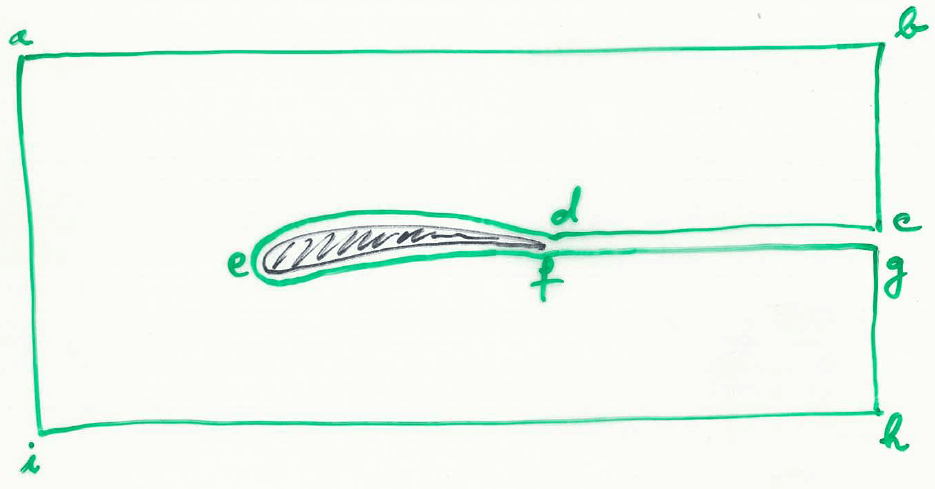
\includegraphics[scale=0.2]{ch4/1}
	\captionof{figure}{}
	\end{wrapfigure}
	The \textbf{autonomous inverters} most of times have bridges composed of fully controllable switches. They can be fed by a DC voltage source (voltage-source converter, VSC) or by a DC current source (current-source converter, CSC). Both models differ on the presence of a capacitor or an inductor in the entry bus. They can work as \textbf{rectifiers}. \textbf{Multi-quadrant} choppers, which are employed to control DC motors, have the same topology and a similar control. 
	
	\begin{minipage}{0.5\textwidth}
		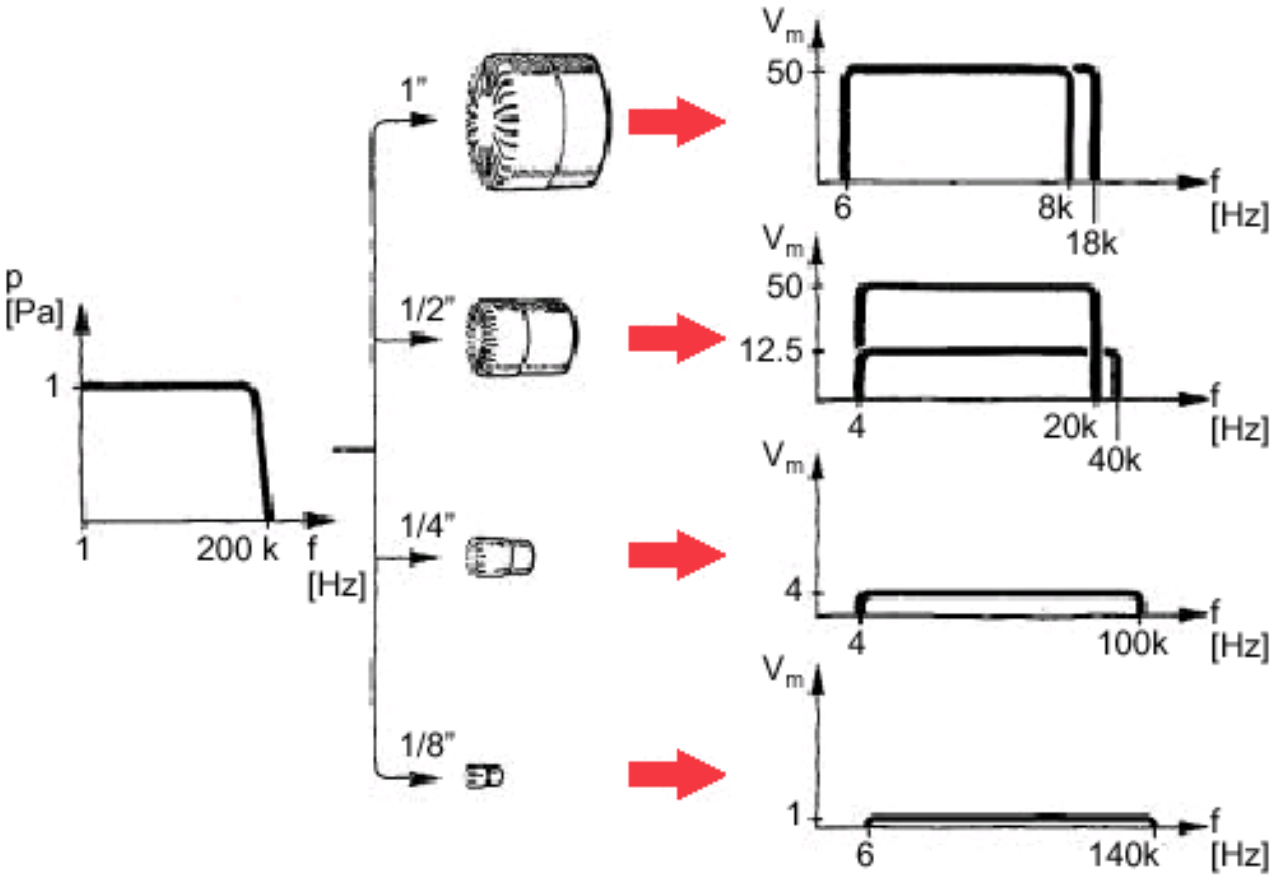
\includegraphics[scale=0.25]{ch4/2}
	\end{minipage}
	\begin{minipage}{0.5\textwidth}
		\vspace{3mm}
		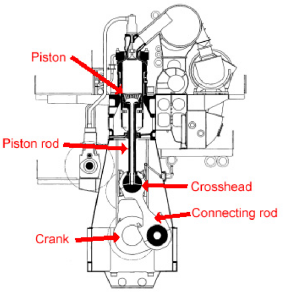
\includegraphics[scale=0.25]{ch4/3}	
	\end{minipage}
	\captionof{table}{List of symbols.}
	
\section{Characteristics of fully controllable switches}
	\begin{wrapfigure}[4]{r}{5 cm}
	\vspace{-5mm}
	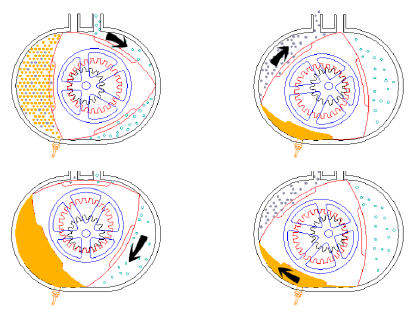
\includegraphics[scale=0.25]{ch4/4}
	\captionof{figure}{}
	\end{wrapfigure}
	Here is the ideal voltage versus current characteristic of a fully-controllable switch. The $2^{nd}$ quadrant doesn't matter to us because the voltage $v_T$ is negative and such an option is left out because there is a diode set in anti-parallel in the switch. \\
	
	\begin{wrapfigure}[6]{l}{6 cm}
	\vspace{-5mm}
	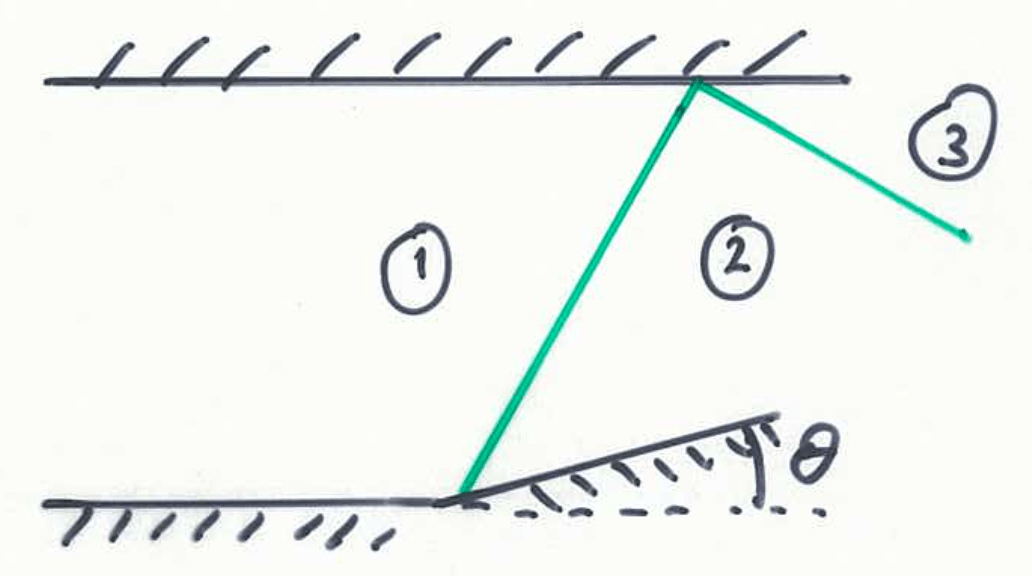
\includegraphics[scale=0.2]{ch4/5}
	\captionof{figure}{}
	\end{wrapfigure}
	All of them are \textbf{unidirectional} and the current cannot flow from the anode A to the cathode K, from the collector C to the emitter E or from the drain D to the source S. The \textbf{control electrode} (trigger G, base B or grid G) allows us to open or close the switch by means of a voltage or current. 
	
	The maximum voltage $V_{T,max}$ and current $I_{T,max}$ the switch can withstand are limited. In order to increase the rated power we can set multiple bridges in parallel or in series but then both the current and the voltage must be evenly distributed. Commutation between conducting and blocking takes a given interval of time that will limit the commutation frequency $f_{s,T}$. During those intervals, current and voltage will be the origin of \textbf{commutation losses}.
	
\section{Voltage-source converters: generalities}
	\subsection{Topologies and practical realisation}	
		\begin{wrapfigure}[12]{l}{7cm}
		\vspace{-5mm}
		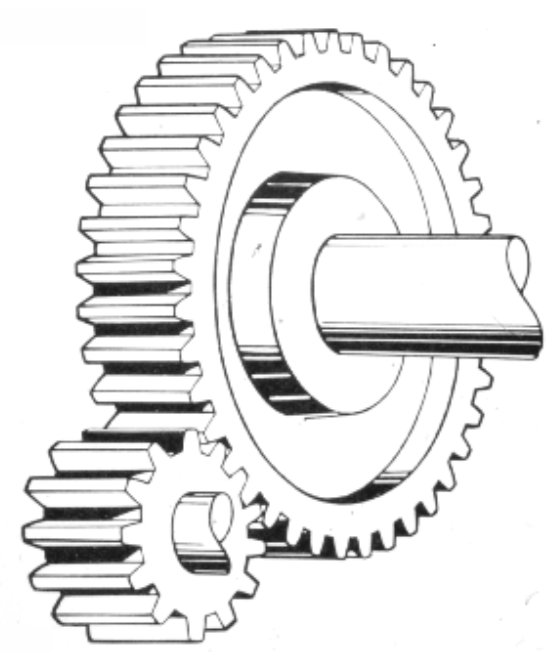
\includegraphics[scale=0.2]{ch4/7}
		\captionof{figure}{}
		\end{wrapfigure}
		This figure represents 4 different bridges with 1,2 or 3 legs. Each leg has a bidirectional fully controllable switch set between the N and P input terminals. The point a, b and c are the output terminals. In the half bridge N and O are also output terminals.
		In order to avoid a short circuit two switches of the same leg cannot be closed at the same time. Otherwise a huge short-circuit current would flow through them and it may destroy them. Depending on which switches are closed and which are open different voltages will appear at the output.\\
		
		For the half bridge without midpoint we have $v_{aN} = 0$ or $v_{aN} = V_{dc}$. In the half bridge with midpoint, $v_{aN} = \pm V_{dc}/2$. In the H-bridge and the three-phase bridge, $v_{aN} = 0$ or $v_{aN} = \pm V_{dc}$. We can therefore create either DC or AC voltages with a chosen average value.  
		
		\begin{wrapfigure}[9]{r}{4cm}
		\vspace{-5mm}
		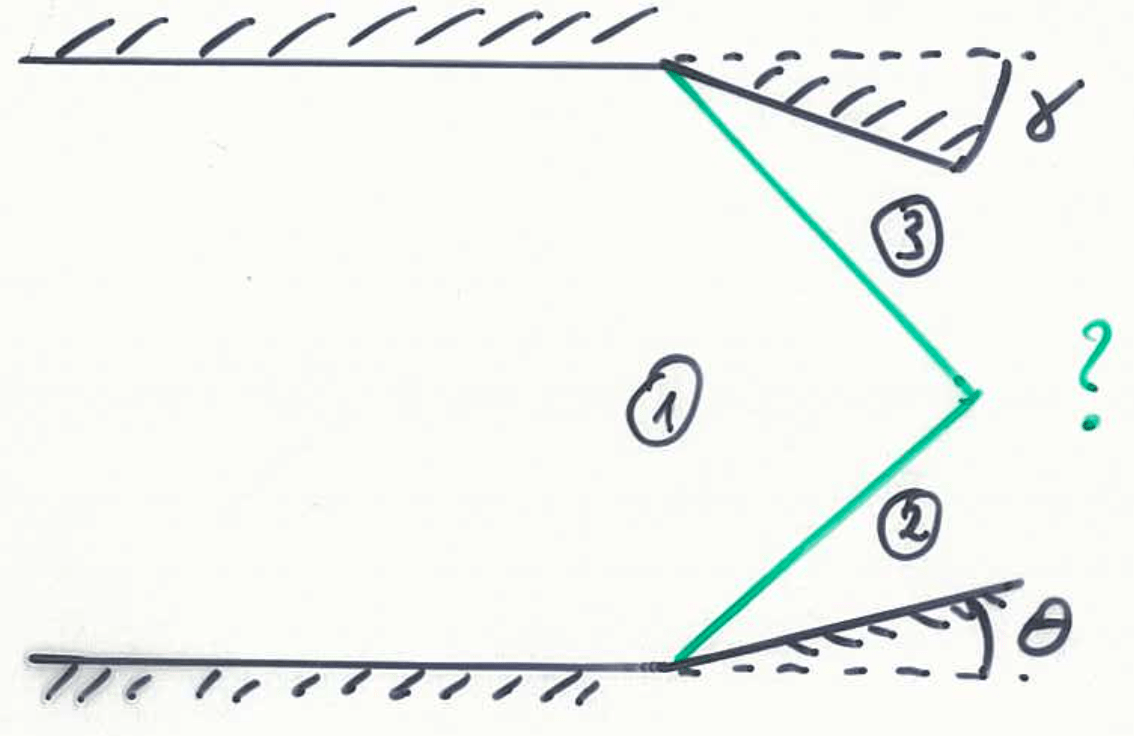
\includegraphics[scale=0.3]{ch4/8}
		\captionof{figure}{}
		\end{wrapfigure}
		\ \\ Here we can observe that each leg is composed of two unidirectional fully controllable switches (GTO, BJT, IGBT, MOSFET, ...), T1 and T2 as well as 2 free-wheeling diodes, D1 and D2 set in anti-parallel with the switches. In order to avoid a short-circuit caused by the diodes, voltage at the input must be \textbf{positive}. If T1 is closed then T2 must be open, a is therefore linked to the P bus and D2 is inversely-biased. If $i>0$, current will not go through T1 but through D1. The same thing happens if T2 is closed, T1 is open and a is linked to the N bus, D1 is inversely biased. If $i>0$ then it won't go through D2 but through T2. \\
		
		Let's focus on $v_{aO}(t)$ of the half bridge while considering $V_{dc}<0$ and constant. Under these conditions, if T1 is closed ($v_{aO(t)} = + V_{dc}/2$) and T2 is closed too ($v_{aO}(t) = -V_{dc}/2$) then for any value of the current $v_{aO}(t)$ depends only on the state of the switches. With an adequate switching frequency T we can get an average output between $+V_{dc}/2$ and $-V_{dc}/2$. \\
		
		As the commutation speed of a switch might be different from the other, there must be an interval of time during which both switches are open at the same times. Otherwise there would be short circuits very often (once every commutation period). We call that time \textbf{dead time} $t_{\Delta}$. During $t_{\Delta}$, the sign of the current will determine $v_{aO}$. 
		
	\subsection{Conduction in the semi-conducting components and associated losses}
		\begin{wrapfigure}[9]{l}{5.5cm}
		\vspace{0mm}
		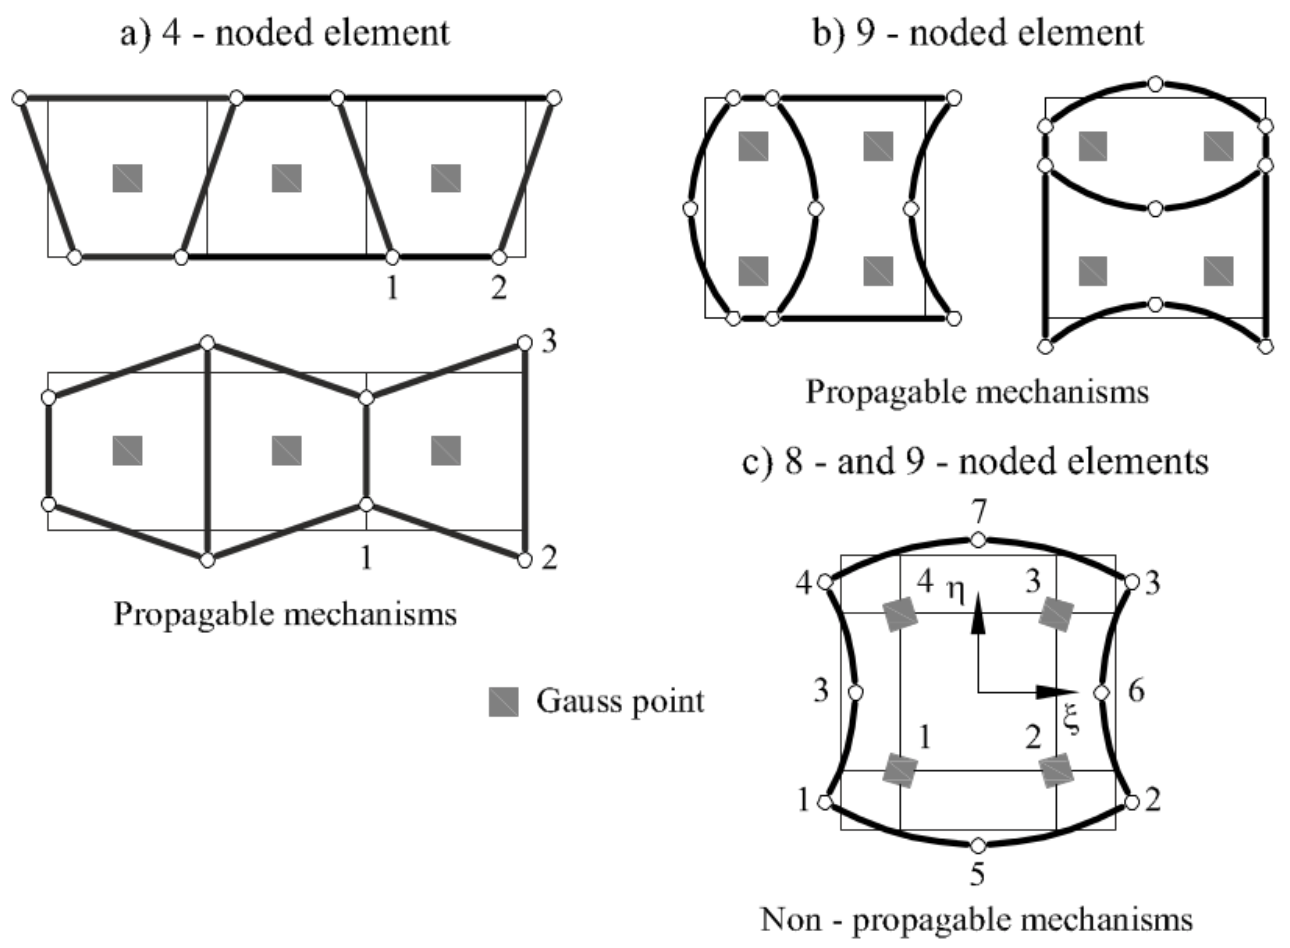
\includegraphics[scale=0.3]{ch4/9}
		\captionof{figure}{}
		\end{wrapfigure}
		When the switches conduct, there is a slight \textbf{residual voltage} at its terminals (1 to 3V). That residual voltage induces a current flow and thus conduction losses. If the switch is open then the leakage current can be neglected.
		In this H-bridge, depending on the state (open or closed) of each switch and the current direction there are up to two times 9 possible combinations (4 $\times$ complementary states, 4 $\times$ a single leg closed). For example, if conduction takes place through D2 and D3 we have:
		\begin{equation}
			V_{ab} = -V_{dc}-V_{F,D2}-V_{F,D3}-(R_{on,D2}+R_{on,D3})i,
		\end{equation}
		where the instantaneous conduction losses (measured in W) are obtained by multiplying the Joule losses term by $i$. When current is negative, it will flow through T2 and T3, and thus:
		\begin{equation}
			V_{ab} = -V_{dc}+V_{F,T2}+V_{F,T3}-(R_{on,T2}+R_{on,T3})i. 
		\end{equation}
		
	\subsection{Commutation in a converter leg and associated losses}
		\begin{wrapfigure}[8]{r}{8cm}
		\vspace{-5mm}
		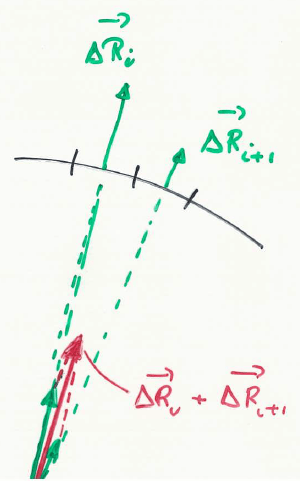
\includegraphics[scale=0.25]{ch4/10}
		\captionof{figure}{}
		\end{wrapfigure}
		Let's consider a half bridge whose midpoint is connected to an inductive load. With such a load current cannot change fast enough and during commutation it will flow through T1 or D2 or both: 
		\begin{equation}
			i = i_{T1}+ i_{D2}.
		\end{equation}		 
		The DC voltage:
		\begin{equation}
			V_{dc} = v_{T1} - v_{D2},
		\end{equation}
		where $v_{T1}$ are $v_{D2}$ near $0$ (in fact they are equal to the threshold voltage) during conduction and equal to $V_{dc}$ and $-V_{dc}$ during non-conduction intervals. During commutation intervals those voltages will go from one value to the other. The waves shapes show that, when T1 is closed, $i_{T1}$ starts increasing from 0 while D2 keeps conducting with $v_{D2} = 0$ and $v_{T1} = V_{dc}$. As long as D2 keeps conducting $-v_{D2}$ cannot rise to $V_{dc}$ and $v_{T1}$ cannot go down to 0. When it opens, $v_{T1}$ must rise 'til $V_{dc}$ in order for D2 to be directly-biased and conduct. \\
		
		During commutation, the instantaneous power consumption $p_{T1} = v_{T1}i_{T1}$ cannot be neglected and the total power consumption will be greater as $V_{dc}, i$ or the commutation intervals increase. As commutation losses are big and problematic the frequency at which those commutations take place will be of great relevance, that frequency is the \textbf{commutation frequency}. We can use the values on the datasheets to calculate the commutation losses in a leg. Those losses can be estimated with this equation:
		\begin{equation}
			P_{com} = f_{s,T} (E_{on,ref}+ E_{off,ref})\frac{V_{dc}}{V_{dc,ref}}\frac{i}{i_{ref}},
		\end{equation}
		where the $E$ are the energies relative to the reference values.
	
\section{Choppers - pulse width modulation (PWM)}
	 \textbf{Pulse width modulation (PWM)} is one of the methods available to control a converter leg. The commutation frequency remains constant and in each leg, the commutation period ($T_{s,T} = 1/f_{s,T}$) is split in 2 parts. During the first part the upper switch is closed and then the lower switch is closed. If we modulate the interval duration of the sub-intervals then we can generate an average voltage. \\
	 
	 The voltages are distorted by lots of harmonics because of commutation. With the aid of inductive loads the current can be rendered smoother. If we control the current through hysteresis, the commutation frequency is not constant and harmonics have a variable frequency. \\
	 In order to do an \textbf{intersective PWM} we have to determine the time when a switch commutes in each leg. We do that by comparing the \textbf{carrier p(t)} (a triangular signal of frequency $f_{s,p}$ and the \textbf{modulator} (the desired voltage). In the single-phase H-bridges we can use the same modulator for both legs (bipolar modulation) or 2 distinct modulators (unipolar modulation) with the same carrier. A \textbf{three-phase} inverter/rectifier has three modulators that constitute a balanced three-phase system. \\
	 
	 When we control the analogical electronics, the comparison between p(t) and m(t) is direct. With numerical electronics, we get the same result without the need of a comparison (duty cycle). 
	 
	 \subsection{Half bridge}
	 	\subsubsection{Without midpoint}
	 		\begin{wrapfigure}[8]{l}{6.5cm}
			\vspace{-5mm}
			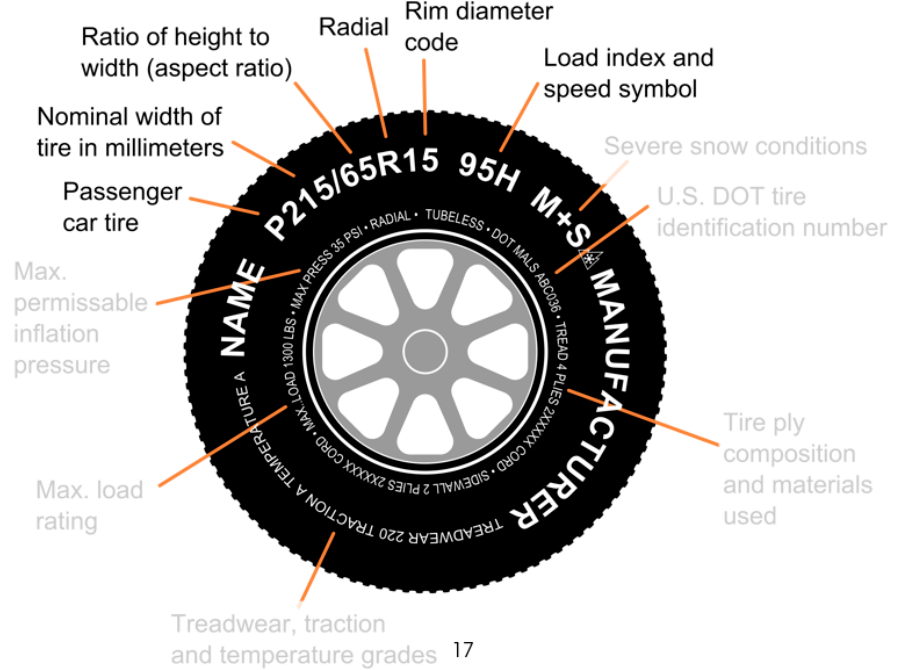
\includegraphics[scale=0.2]{ch4/6}
			\captionof{figure}{}
			\end{wrapfigure}
			
			As the output voltage $v_{aN}(t)$ is always either positive or null, we use a triangular carrier p(t) that varies between 0 and 1. The modulator m(t) should change slowly (constant over a commutation period $T_{s,p}$) with respect to the carrier. When $m(t) > p(t)$, the upper switch of the leg is closed and $v_{aN} = V_{dc}$. When $m(t) < p(t)$, the closed switch is the closed one $v_{aN} = 0$. We consider that m(t) will also fluctuate between 0 and 1 in such a way that p and m intersect each other twice by commutation period $T_{s,p}$ and the switches will open and close themselves at the same frequency. We also find that frequency in $v_{aN}$ : 
			\begin{equation}
				f_{s,p} = f_{s,T} = f_{s,v}. 
			\end{equation}
			We will introduce a new parameter, the \textbf{duty cycle} of the switch. The duty cycle is the fraction of time during which the switch is closed ($0<D_x<1$). If we neglect the dead time of the switches: 
			\begin{equation}
				D_1 = \frac{T_{on,1}}{T_s} \qquad and \qquad D_2 = \frac{T_{on,2}}{T_s} = \frac{T_s - T_{on,1}}{T_s} = 1 - D_1.
			\end{equation}
			By convention, D (without any number) is the duty cycle of the upper switch, that is to say $D = D_1$. In this case:
			\begin{equation}
				D(t) = m(t). 
			\end{equation}
			We will do a \textbf{fast average} of $v_{aN}$ (average without commutation harmonics) as follows: 
			\begin{equation}
				V_{aN}(t) = \frac{1}{T_s}\int _{t-T_s/2}^{t+T_s/2} v_{aN}(t') \, dt'
			\end{equation}
			This average will change slowly with respect to $T_s$. It will be (approximately): 
			\begin{equation}
				V_{aN}(t) = m(t) V_{dc}. 
			\end{equation}
			
		\subsubsection{With midpoint}
			As $V_{aO}(t) = V_{aN}(t) - V_{dc}/2$ can be either positive or negative, this bridge can operate as an inverter/rectifier and as a chopper. If we take the same $p(t)$, we will always have $D(t) = m(t)$ and:
			\begin{equation}
				V_{aO}(t) = V_{aN}(t) - V_{dc}/2 = (m(t) - \frac{1}{2})V_{dc} \qquad and \qquad f_{s,p} = f_{s,T} =f_{s,v}
			\end{equation}
			
	\subsection{H-bridge}
		\subsubsection{Bipolar modulation}
		    In this case, we only need to use a single carrier $p(t)$ and a single modulator $m(t)$. If we control the switches diagonally ($T^a$ with $T_b$ and $T_a$ with $T^b$). This way, $v_{ab}(t)$ is either $V_{dc}$ or $-V_{dc}$. We have \textbf{bipolar commutation} because we combine 2 voltages. Diagonal commutation implies $v_{bO}(t) = - v_{aO}(t)$ and an output equal to twice that of half bridge with midpoint:
			\begin{equation}
				v_{ab}(t) = v_{aO}(t)-v_{bO}(t) = 2v_{aO}(t) \qquad \Rightarrow \qquad V_{ab}(t) = (2D(t)-1)V_{dc} = m(t) V_{dc},
			\end{equation}
			where D(t) is the duty cycle of the first leg. All the 3 $f_s$ are always equal.
			
		\subsubsection{Unipolar modulation}
			\begin{wrapfigure}[14]{l}{8cm}
			\vspace{-5mm}
			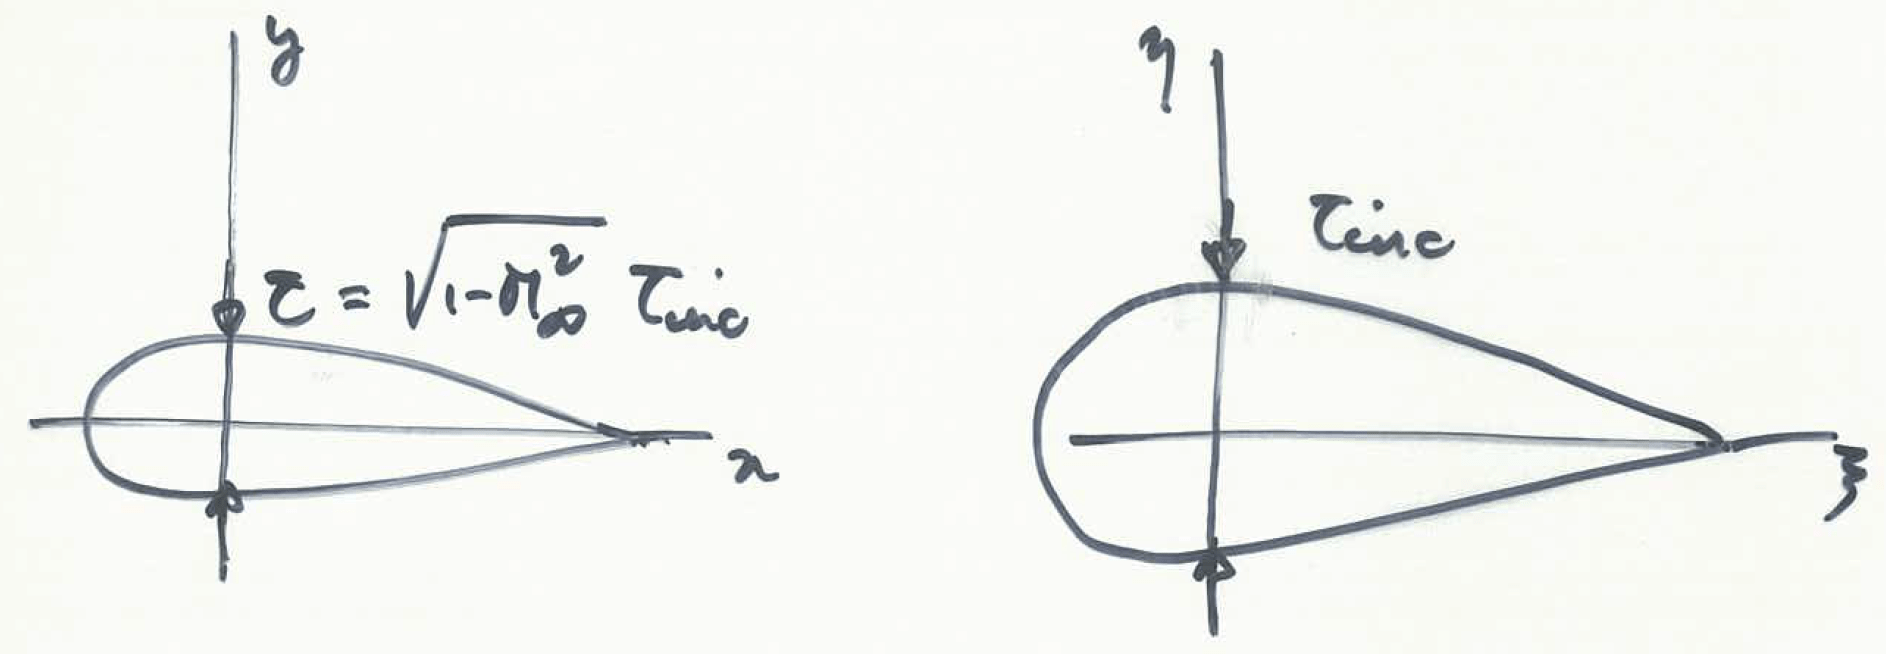
\includegraphics[scale=0.25]{ch4/11}
			\captionof{figure}{}
			\end{wrapfigure}
			We can also employ different modulators $m(t)$ for each leg. The carrier $p(t)$ will fluctuate between -1 and 1, with a modulator $m(t)$ for the control of the first leg and $-m(t)$ for the control of the second leg. When $m(t) > 0$, $v_{ab}(t)$ has positive impulsions of amplitude $V_{dc}$ ny commutation period. Therefore:
			\begin{equation}
				2 f_{s,p} = 2f_{s,T} = f_{s,v}.
			\end{equation}
			Let's note that there are intervals with a null output (the load is short-circuited). The output voltage is the same as before. \\
			
		\subsubsection{Bipolar versus unipolar modulation}
			\begin{wrapfigure}[8]{r}{7cm}
			\vspace{-5mm}
			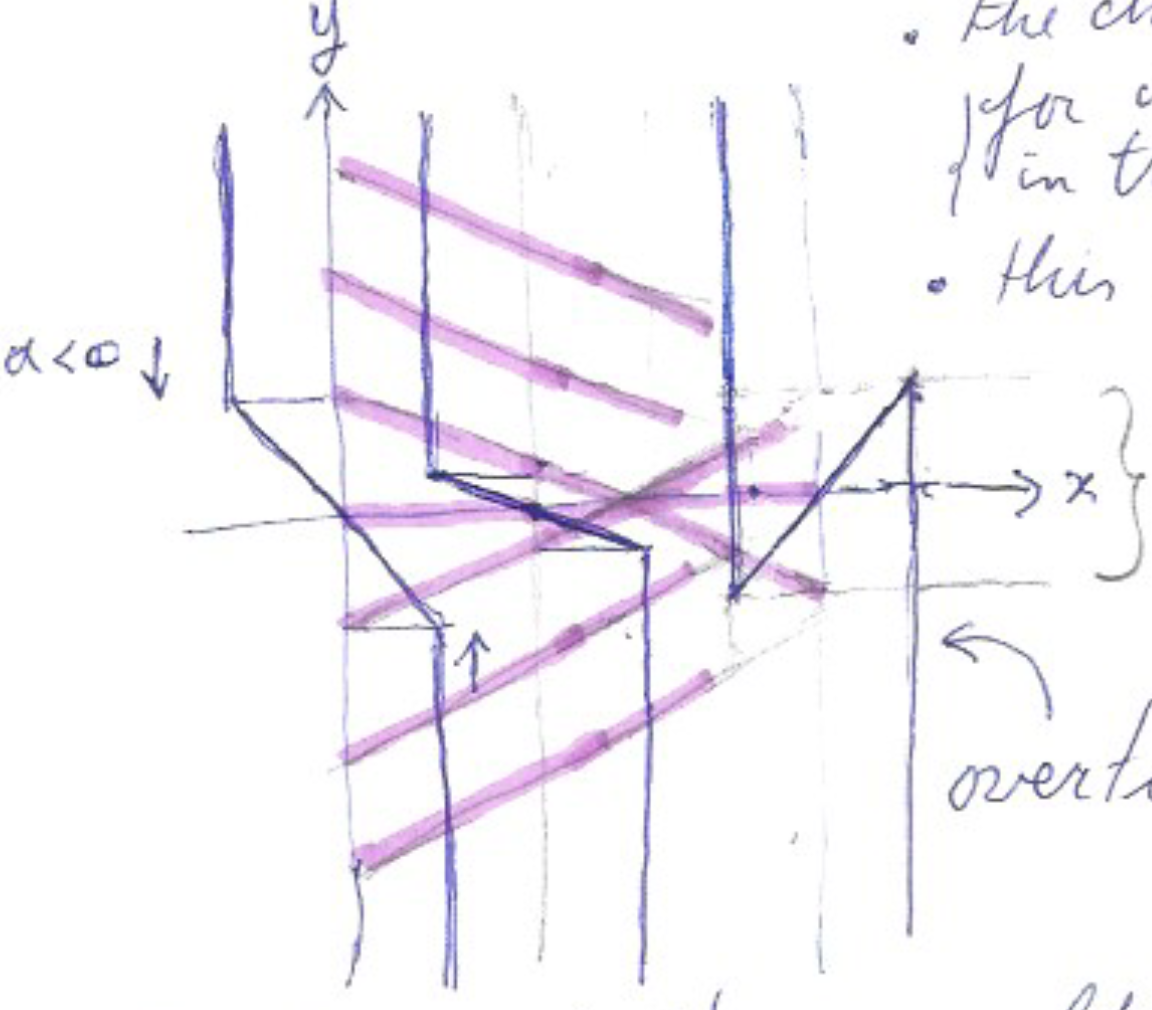
\includegraphics[scale=0.2]{ch4/12}
			\captionof{figure}{}
			\end{wrapfigure}
			In the case of a bipolar modulation, there is a positive impulsion with length $DT_{s,T}$ and a negative impulsion $(1-D)T_{s,T}$ each commutation interval. If we have an unipolar modulation, then there are two impulsions with the same sign during each commutation period. The difference between both cases will be grow bigger as $|D-0.5|$ grows smaller.
			\newpage
			
	\subsection{Coverage in the voltage versus current plan}
		\begin{wrapfigure}[10]{l}{7.5cm}
		\vspace{-5mm}
		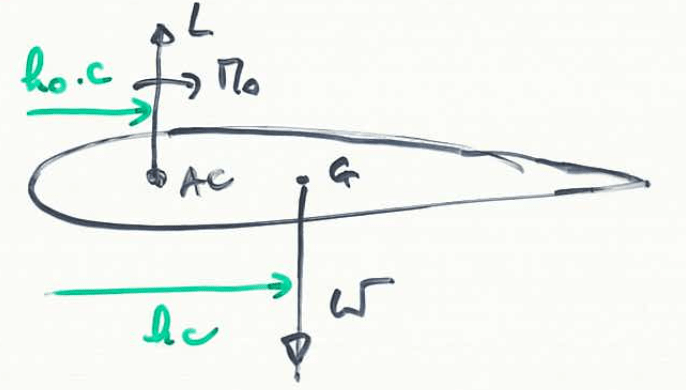
\includegraphics[scale=0.28]{ch4/13}
		\captionof{figure}{}
		\end{wrapfigure}
		\textbf{Choppers} carry out DC-DC conversions between a positive voltage $V_{dc}$ at the input and an average output that can be either positive or negative $V_{aN}, V_{aO}$ or $V_{ab}$. There is no constraint over the sign of $i(t)$ but there is a constraint on its average value: $-I_{T,min}\leq I \leq I_{T,max}$. Depending on its sign and that of the output voltage the power flow will go in one direction or the other. We can therefore distinguish 4 operation quadrants in the voltage versus current plan of choppers. 
		
	\subsection{Inductive load, distortion of the output current}
		\begin{wrapfigure}[8]{r}{9cm}
		\vspace{-5mm}
		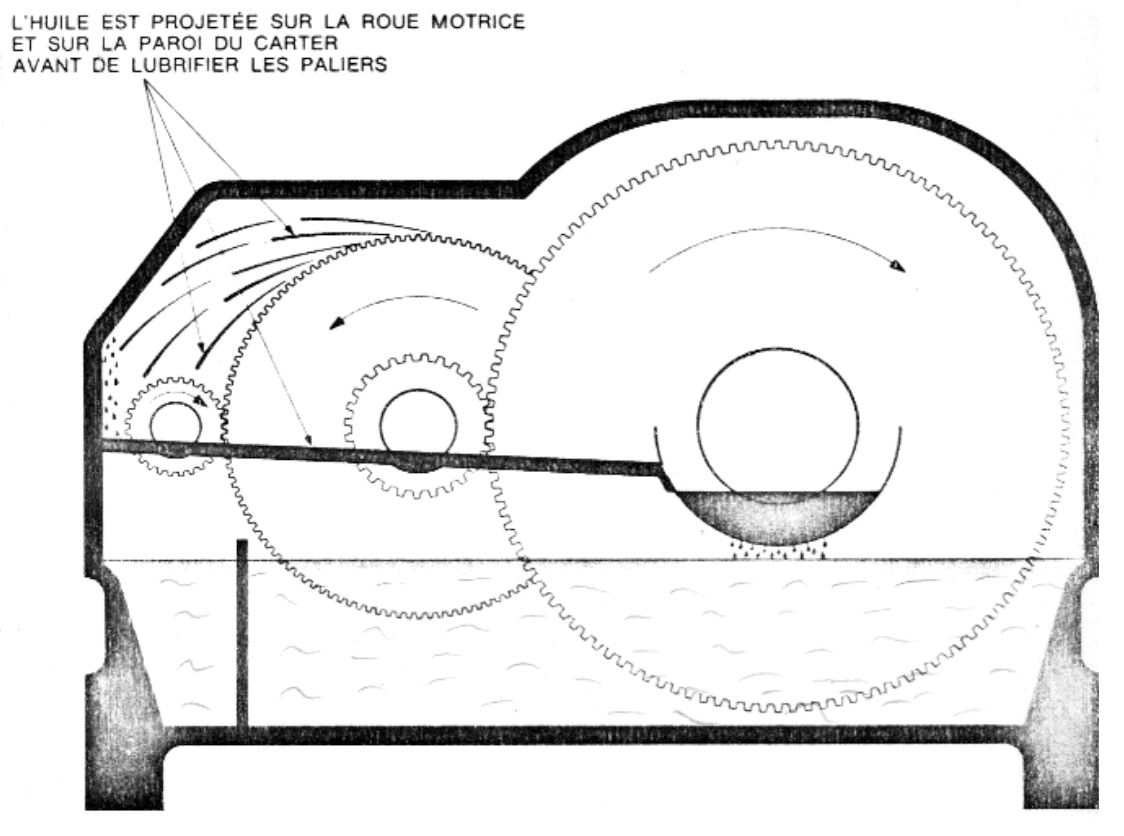
\includegraphics[scale=0.25]{ch4/14}
		\captionof{figure}{}
		\end{wrapfigure}
		If the chopper has an RLE load fed by a voltage fluctuating between $V_{min}$ and $V_{max}$, with a period a period $T_{s,v}$ that depends on $f_{s,T}$ and the PWM employed. We consider a simplified system at steady-state and with a voltage $E=cst$. The instantaneous and average values are related by the following equations:\\
		\begin{equation}
			v(t) = Ri(t) + L\frac{di}{dt} + E \qquad and \qquad V = RI + E.
		\end{equation}
		If we subtract these equations we find the variations:
		\begin{equation}
			\Delta v(t) = R\delta i(t) + L\frac{d\Delta i}{dt}.
		\end{equation}
		$\Delta v(t)$ is constant during each interval and its value is $\Delta V_{max}$ during an interval $T_{v,max}$ and $\Delta V_{min}$ during $T_{v,min}$, with $T_{v,min} + T_{v,max} = T_{s,v}$. As the average $\Delta v(t) = 0$, we have:
		\begin{equation}
			\Delta V_{max}T_{v,max} + \Delta V_{min}T_{v,min} = 0 \qquad with \qquad \Delta V_{max} \geq 0 \ and \ \Delta V_{min} \leq 0
		\end{equation}
		$i(t)$ has sawtooth shape. Its rising slopes last $T_{v,max}$ and their descent lasts $T_{v,min}$. If the time constant $\tau = L/R \gg T_{s,v}$, the slope of the sides is almost constant and equals either $\Delta V_{max}/L$ or $\Delta V_{min}/L$. The peak-to-peak ripple $\Delta i(t)$ and $i(t)$ are:
		\begin{equation}
			\Delta I_{pp} = \frac{\Delta V_{max}T_{v,max}}{L} = -\frac{\Delta V_{min}T_{v,min}}{L}.
		\end{equation}
		
		The increase of $I_{rms}$ because of the ripple can be calculated as follows:
		\begin{equation}
		\begin{array}{c}
			I_{rms} = \sqrt{I^2+(\Delta I_{rms})^2} \qquad with \\
			\Delta I_{rms} = (\Delta i)_{rms} = \sqrt{\frac{1}{T_{s,v}}\int _{t_0}^{t0+T_{s,v}}(\Delta i)^2\, dt} = \Delta I_{pp} \sqrt{\int _{-1/2}^{1/2}x^2\, dx} 
		\end{array}
		\end{equation}
		Finally:
		\begin{equation}
			\Delta I_{rms} = \frac{1}{2\sqrt{3}}\Delta I_{pp}.
		\end{equation}
		Additional Joule losses in the loads' resistance R are $R(\Delta I_{rms})^2$. \\
		
		\textbf{Half bridge without midpoint} \qquad We have $T_{s,v} = T_{s,T}$, $V_{aN} = DV_{dc}, T_{v,max} = DT_s, \Delta V_{max} = V_{dc}-V_{aN}= (1-D)V_{dc}$ and thus:
		\begin{equation}
			\Delta I_{pp} = (1-D)D\frac{V_{dc}}{f_{s,T}L}= (1-D)\frac{V_{aN}}{f_{s,T}L}. 
		\end{equation}
		We can therefore decrease the ripple by increasing L and/or $f_{s,T}$. That ripple will also depend on D and it will reach a maximum for D = 0.5. \\
		
		\textbf{Half bridge with midpoint} \qquad We have $T_{s,v} =T_{s,T}, V_{aO} = (2D-1)V_{dc}/2, T_{v,max}=DT_{s,T}, \Delta V_{max} = V_{dc}/2-V_{aO = (1-D)V_{dc}}$ and thus:
		\begin{equation}
			\Delta I_{pp} = (1-D)D\frac{V_{dc}}{f_{s,T}L} = \frac{2(1-D)D}{2D-1}\frac{V_{aO}}{f_{s,T}L}.
		\end{equation}
		\ \\
		
		\textbf{H-bridge and bipolar topology}\qquad We have $T_{s,v} = T_{s,T}, V_{ab}=(2D-1)V_{dc}, T_{v,max}=DT_{s,T}, \Delta V_{max}= V_{dc}-V_{ab}=2(1-D)V_{dc}$ and thus:
		\begin{equation}
			\Delta I_{pp} = 2(1-D)D\frac{V_{dc}}{f_{s,T}L} = \frac{2(1-D)D}{2D-1}\frac{V_{ab}}{f_{s,T}L}.
		\end{equation}
		
		\ \\ \textbf{H-bridge and unipolar topology} \qquad If we consider a positive average voltage ($0.5\leq D\leq 1$) $T_{s,v} = T_{s,T}/2, V_{ab} =(2D-1)V_{dc}\geq 0, V_{max}=V_{dc}, T_{v,max}=(D-0.5)T_{s,T}, V_{min}=0, T_{v,min}= (1-D)T_{s,T}, \Delta V_{max}= V_{dc}-V_{ab}=2(1-D)V_{dc}$ and thus:
		\begin{equation}
			\Delta I_{pp} = (1-D)(2D-1)\frac{V_{dc}}{f_{s,T}L} = (1-D)\frac{V_{ab}}{f_{s,T}L}
		\end{equation}
		
		For a negative average voltage ($0\leq D\leq 0.5$) $T_{s,v} = T_{s,T}/2, V_{ab} =(2D-1)V_{dc}\leq 0, V_{max}=0, T_{v,max}=DT_{s,T}, V_{min}=-V_{dc}, T_{v,min}= (0.5-D)T_{s,T}, \Delta V_{max}= 0-V_{ab}=(1-2D)V_{dc}$ and:
		\begin{equation}
			\Delta I_{pp} = D(1-2D)\frac{V_{dc}}{f_{s,T}L} = D\frac{-V_{ab}}{f_{s,T}L}.
		\end{equation}
		The current produced by an unipolar modulation is less distorted than the one produced by a bipolar modulation if we have a duty cycle distanced from the extreme cases D = 0 or D=1. The greater difference appears when D=0.5. These expressions are valid for the transient signal as long as we can split the fundamental variation of the quantities and the variation due to to commutations.
		
	\subsection{Dead time}
		\begin{wrapfigure}[7]{l}{7cm}
		\vspace{-5mm}
		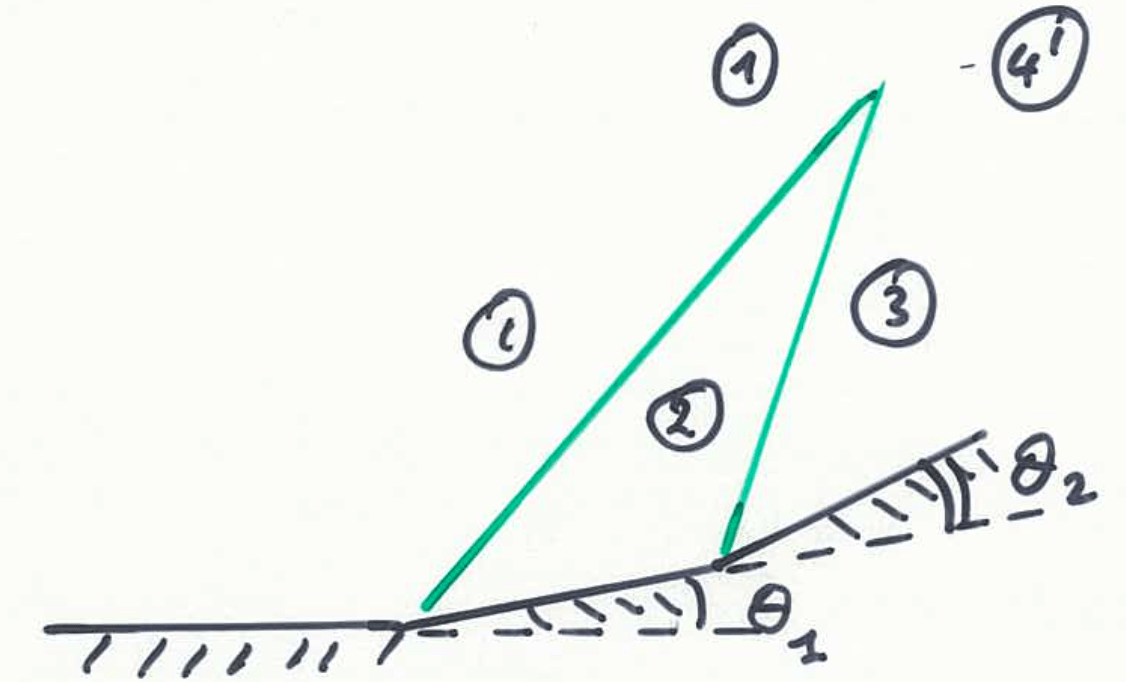
\includegraphics[scale=0.2]{ch4/15}
		\captionof{figure}{}
		\end{wrapfigure}
		In practice, we have a short interval during which both switches are open in order to avoid a short-circuit during commutations. In the case of a \textbf{half bridge}, during the instants at which T1 and T2 are open simultaneously, the sign of $i$ determines the value of $v_{aN}$. If $i>0$, it will flow through D2 and $v_{aN} =0$. If $i<0$, it will flow through D1 and
		
		\newpage $v_{aN} = V_{dc}$. The figure shows what happens to the output voltage when the \textbf{turning-on of the switches} is delayed by $t_{\Delta}$. This is only valid if the load is inductive. Otherwise the current $i$ would be less smooth and it might get inverted. 
		
\section{Single-phase voltage-source inverters}
	\begin{wrapfigure}[10]{l}{10cm}
	\vspace{-5mm}
	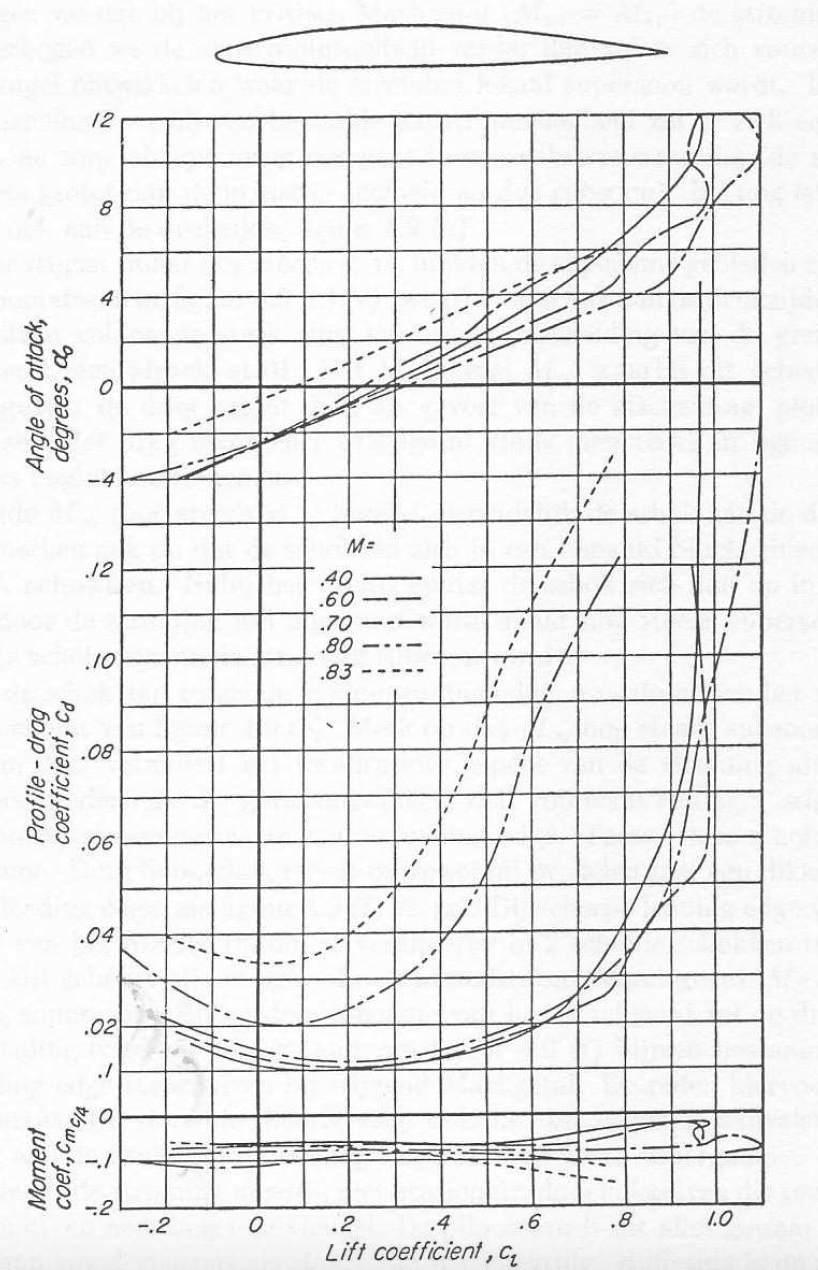
\includegraphics[scale=0.28]{ch4/16}
	\captionof{figure}{}
	\end{wrapfigure}
	They consist of 1 or 2 legs. A half bridge must have a midpoint linked to the source. If needed we can create it using tow condensers with the same capacity C(which must be high). In the case of an H-bridge that is not necessary. In practice, the inverter is fed by a rectifier (that is why we need the capacitor at the input). If the source is a battery, the capacitor takes over the AC component of the current and mitigates the effect of the inner resistance while the battery furnishes the average voltage(component?).
	
	\subsection{Linear sinusoidal PWM}
		\subsubsection{Half bridge}
			\begin{wrapfigure}[14]{r}{7cm}
			\vspace{-5mm}
			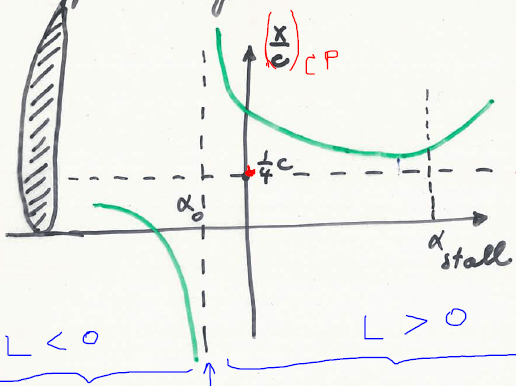
\includegraphics[scale=0.28]{ch4/17}
			\captionof{figure}{}
			\end{wrapfigure}
			We choose a triangular signal of frequency $f_{s,p}$ as the carrier$p(t)$. The carrier will fluctuate between -1 and 1. On the other hand, the modulator $m(t)$ will be a sinusoid of frequency $f$ and amplitude $\hat{m}$, image of the desired voltage. The \textbf{phase angle} is the third degree of freedom of $m(t)$. We will introduce the \textbf{amplitude index}. The amplitude index is the ratio of the peak voltages:
			\begin{equation}
				\hat{m} = \frac{\hat{m}}{1}
			\end{equation}
			If we first consider the amplitude index to be $<1$, then we can introduce the \textbf{frequency index}: 
			\begin{equation}
				m_f = \frac{f_{s,p}}{f}.
			\end{equation}
			It should be an \textbf{integer} (synchronous PWM) and in the case of a half bridge an odd integer). If $m_f$ is an even integer then $v_{aO}(t)$ has half-wave symmetry $v_{aO}(t) = - v_{aO}(t+T/2)$ (no even order harmonics). When $\hat{m}\leq 1$, m(t) and p(t) intersect twice by commutation period $T_{s,T} = T_{s,p}$.\\
			
			 If $m_f$ is big enough (e.g. $\geq 9$) m(t) changes slowly in comparison with p(t) and the problems we with the choppers are relevant once again. Thus the amplitude of the fundamental $\hat{V}_{aO,1}$ is: 
			 \begin{equation}
			 	\hat{V}_{aO,1} = \hat{m}\frac{V_{dc}}{2}.
			 \end{equation}
			 We call it \textbf{linear modulation}. Besides the fundamental component of the fundamental frequency $f$, the voltage comprises high even-order harmonics $h = km_f \pm l$ with $k=1,2,...$ and $l$ integer and small. 
			
		\subsubsection{H-bridge}
			\begin{wrapfigure}[16]{l}{5cm}
			\vspace{-5mm}
			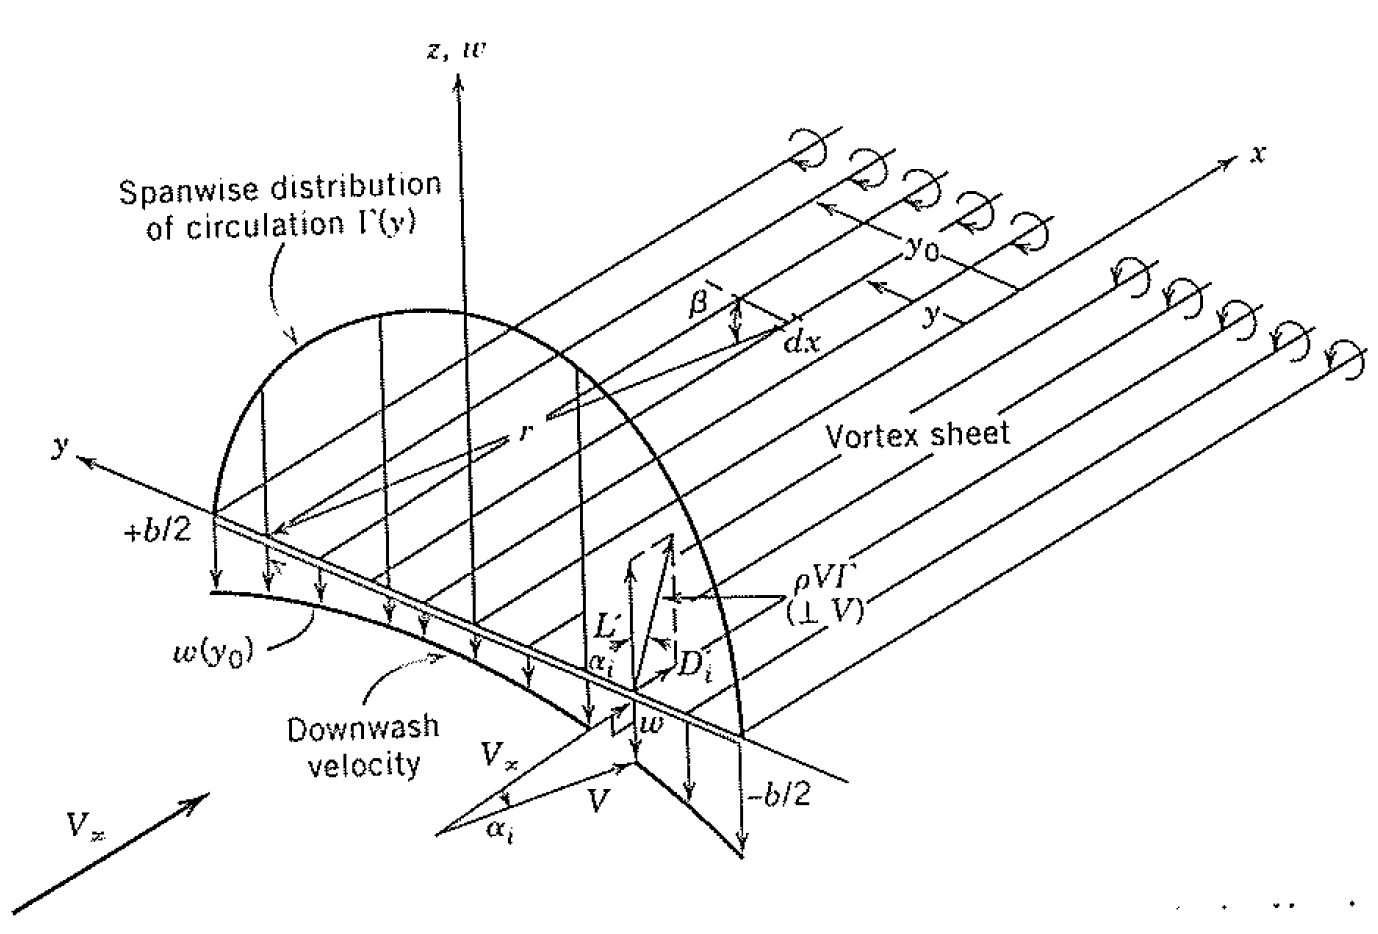
\includegraphics[scale=0.28]{ch4/18}
			\captionof{figure}{}
			\end{wrapfigure}
			Once again we must distinguish the bipolar from the unipolar case. But, for both the output voltage is:
			\begin{equation}
				\hat{V}_{ab,1} = \hat{m}V_{dc}. 
			\end{equation}
			\textbf{Bipolar PWM} \qquad The final wave-shape is the same as with the half-bridge except it varies between $-V_{dc}$ and $+V_{dc}$. Remember: $m_{f}$ should be integer and odd, that way the spectre has way less components. 
			
			\paragraph{Unipolar PWM} \quad  The figure shows that the impulsions are either positive or negative (between 0 and $\pm V_{dc}$) during positive and negative alternations of $m(t)$ respectively. This time $m_f$ should be integer and even. That way the output has half-wave symmetry. The order of harmonics is given by $h=2km_f \pm l$. The commutation frequency has doubled $\Rightarrow$ good for the current ripple with big $L$. 
			
	\subsection{Overmodulation and square-wave switching}
\begin{center}
		\begin{minipage}{0.45\textwidth}
			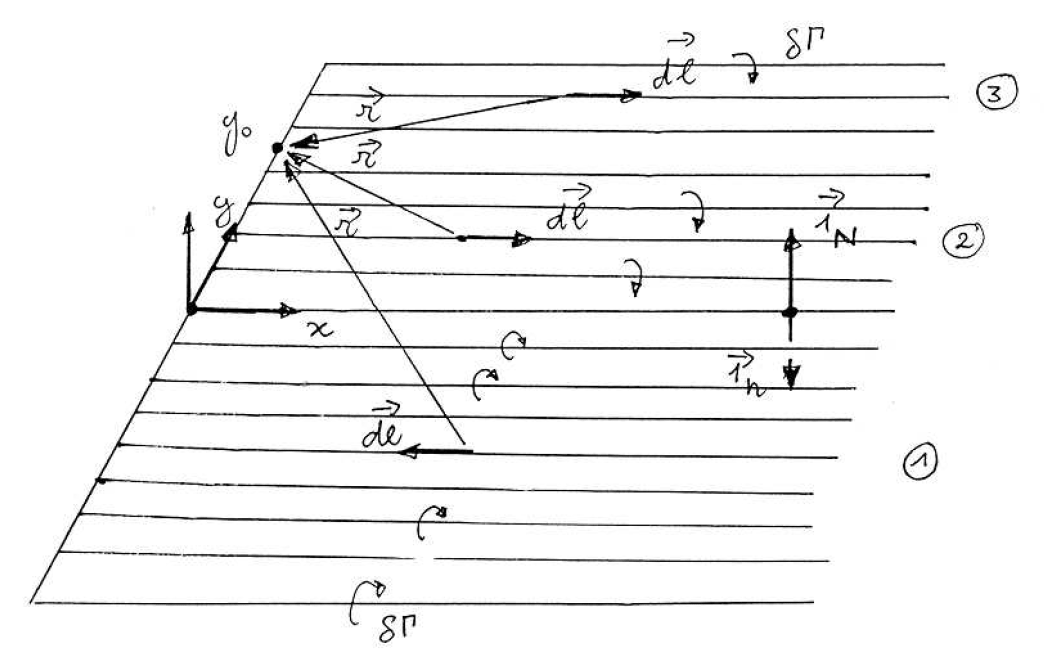
\includegraphics[scale=0.25]{ch4/19}
			\captionof{figure}{}
		\end{minipage}
		\begin{minipage}{0.45\textwidth}
			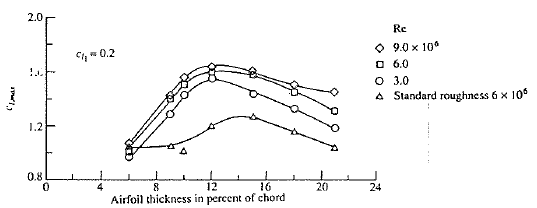
\includegraphics[scale=0.4]{ch4/20}
			\captionof{figure}{}
			\label{fig:4.18}
		\end{minipage}
\end{center}

		Overmodulation appears when $\hat{m}>1$. If we have overmodulation there are less commutations by fundamental period T because p(t) and m(t) intersect each other less often. That means that there will be less commutation losses. The commutation frequency with overmodulation is limited: $f < f_{s,T} < f_{s,p}$. In the figure we can see that the amplitude of the signal doesn't vary linearly with $\hat{m}$ and low order harmonics begin to appear 
		
		\paragraph{The square wave}\quad For $\hat{m}$ bigger than a certain limit that depends on $m_f$ (integer), the intersection will only take place when $m(t)=0$ and we have a square wave of whose fundamental voltage amplitude is maximal (\autoref{fig:4.18}):
		\begin{equation}
			\hat{V}_{1} = n_b \frac{4}{\pi}\frac{V_{dc}}{2}. 
		\end{equation}		  
		where $n_b = 1$ or $n_b = 2$ depending on the topology of the bridge, half bridge or bipolar H-bridge. Each switch is open or closed only once by period T. The switching frequency $f_{s,T} = f$ is minimal, which allows us to use slow switches such as GTOs (minimal losses). In a square-wave voltage $V_1$ is maximal but it must be regulated via $V_{dc}$. Therefore, we need a \textbf{controlled rectifier} set upstream (instead of the cheap diode rectifier). Presence of low order harmonics is another problem. \\
		
		The linear PWM requires faster switches. In addition, bigger $m_f$ implies faster commutations and thus more commutation losses. However, we can change $\hat{V}_1$ by modifying $\hat{m}$. As they are high order harmonics, current harmonics have low amplitudes (if the load is inductive). 
		
	\subsection{Generic RLE load and fundamental and harmonic components of the current}
		\begin{wrapfigure}[8]{l}{7.5cm}
			\vspace{-5mm}
			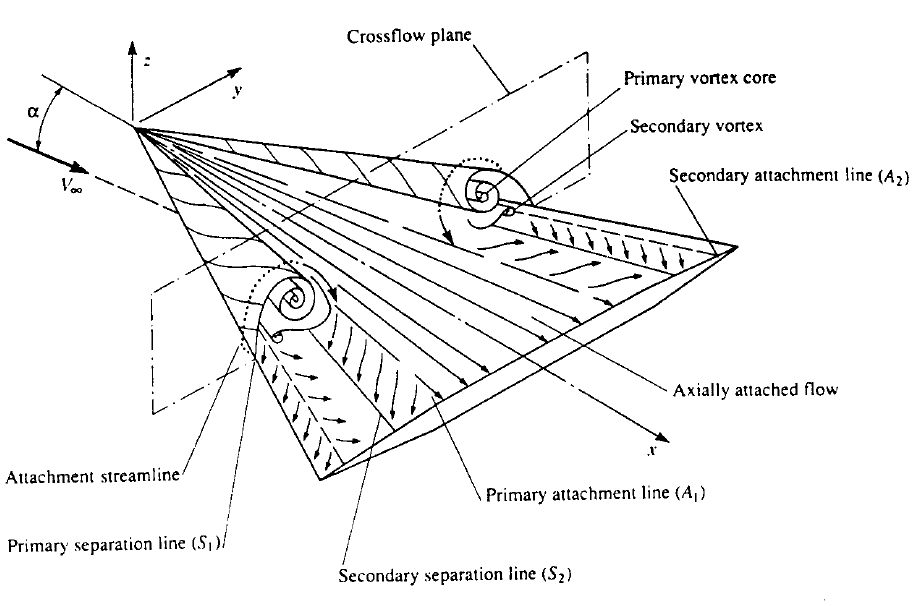
\includegraphics[scale=0.25]{ch4/21}
			\captionof{figure}{}
			\end{wrapfigure}
			If we consider an RLE load with an e.m.f source, the $e(t) = \sqrt{2}E\cos (\omega t + \gamma _e)$. It might also be a single-phase grid and its Thevenin-equivalent. In practice, the reactance $R\ll X = \omega L$ to the fundamental pulsation and the distortion of $e(t)$ are neglected. Having the same pulsation for $e(t)$ and the fundamental value of the output voltage $v_1(t) = \sqrt{2}V_1 \cos (\omega t +\gamma _{v,1})$ is essential. In steady-state the fundamental value of the current $i_1(t)$ in the load has the same pulsation $\omega$. We can represent those 3 quantities as functions of phasors as follows:
			\begin{equation}
				\underline{E} = Ee^{j\gamma _e}, \underline{V}_1 = V_1e^{j\gamma _{v,1}}, \underline{I}_1 = I_1e^{j\gamma _{i,1}} \qquad \underline{V}_1=\underline{E}+(R+j\omega L)\underline{I}_1
			\end{equation}
			If we isolate the current in this equation:
			\begin{equation}
				\underline{I}_1 = \frac{\underline{V}_1-\underline{E}}{R+j\omega L}.
			\end{equation}
			We ascertain that if we act in the phase angle and the amplitude of $v_1(t)$, we can control $i_{1}(t)$ and thus the active and reactive power flux. In the figure here, there are two different cases. First, when $\underline{I}_1$ is in-phase with $\underline{E}$. Second, it is in counter-phase with $\underline{E}$. The circuit will behave as a load and as a source respectively. 
			
			\paragraph{Current harmonics} \quad As for $h>1$, $\underline{E}_h =0$, the rms values of harmonics $\underline{I}_h$ are: 
			\begin{equation}
				\underline{I}_h = \frac{\underline{V}_h}{\sqrt{R^2+(h\omega L)^2}} \approx \frac{\underline{V}_h}{h\omega L}. 
			\end{equation}
			The mitigation of the current due to the inductance improves with the order and the pulsation $h\omega$. Low order harmonics (h=3, 5, ...) are slightly mitigated. 
			
\section{Three-phase voltage-source inverters}
	\subsection{Linear sinusoidal PWM}
		\begin{wrapfigure}[7]{r}{5.5cm}
		\vspace{-5mm}
		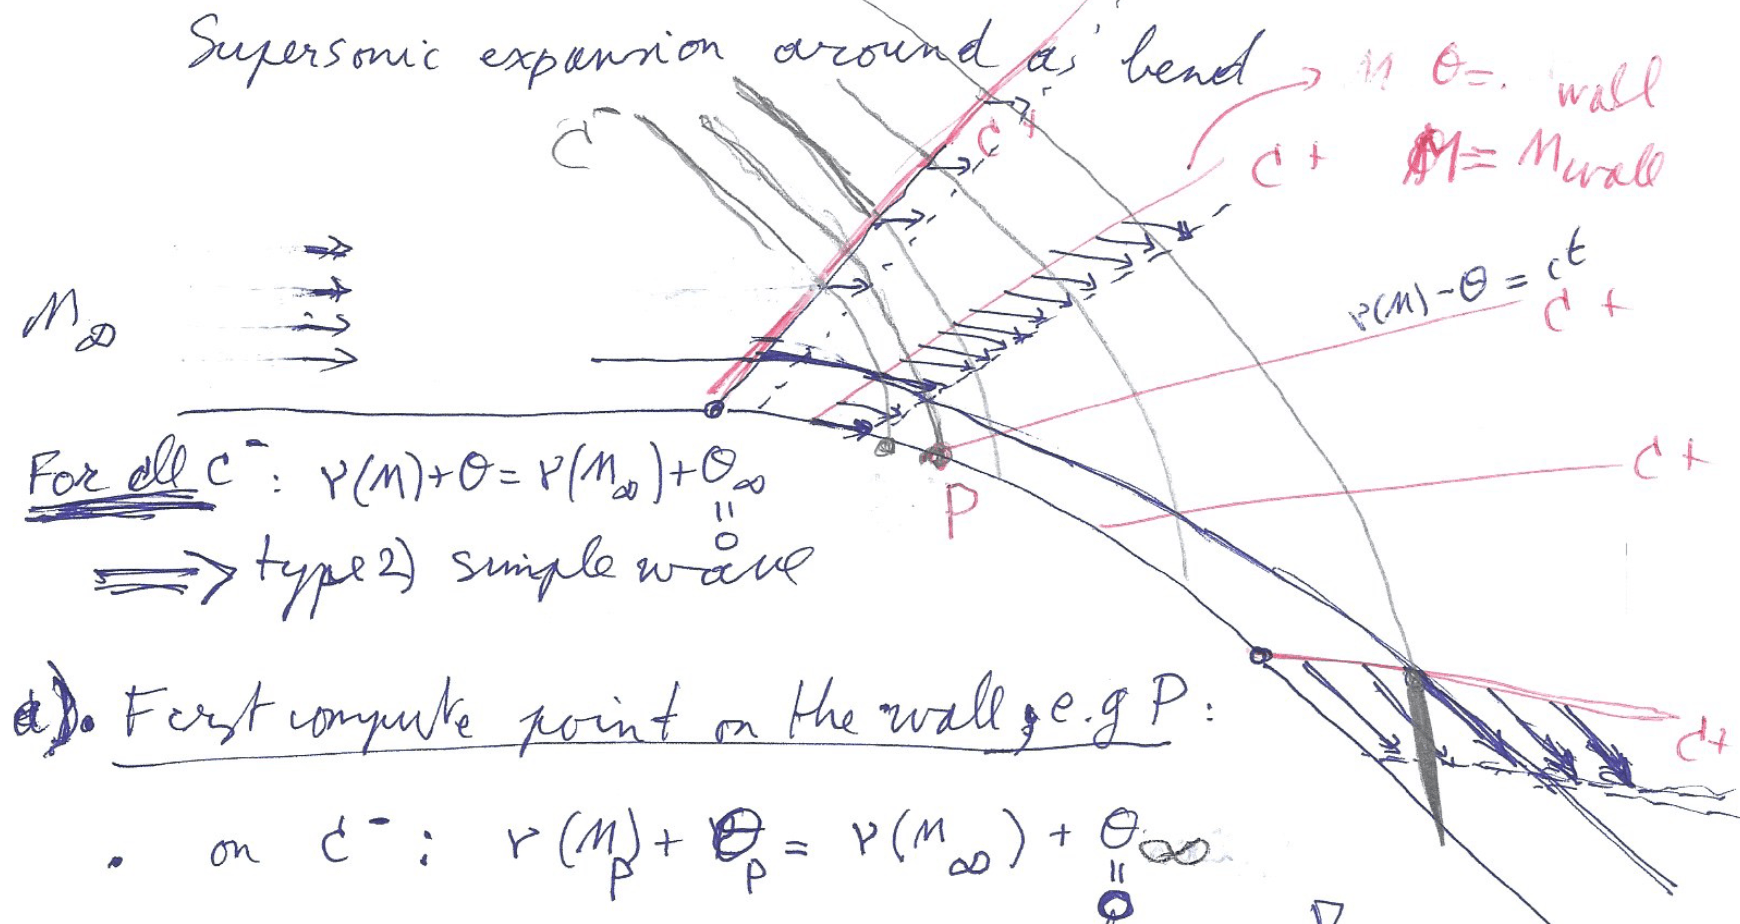
\includegraphics[scale=0.25]{ch4/22}
		\captionof{figure}{}
		\end{wrapfigure}
		Now we have 3 legs and the load is connected to the 3 midpoints a, b and c. The midpoint O of the DC bus makes the equations easier to write but is not necessary for the inverter to work. For a linear modulation, the control of the 6 switches is made by comparing a carrier $-1< p(t)<1$ with frequency $f_{s,p}$ and 3 modulators $m(t)$ that constitute a three-phase system of frequency $f$, amplitude $\hat{m}_a=\hat{m}_b=\hat{m}_c$ and 
		
		\begin{wrapfigure}[11]{l}{4cm}
		\vspace{-5mm}
		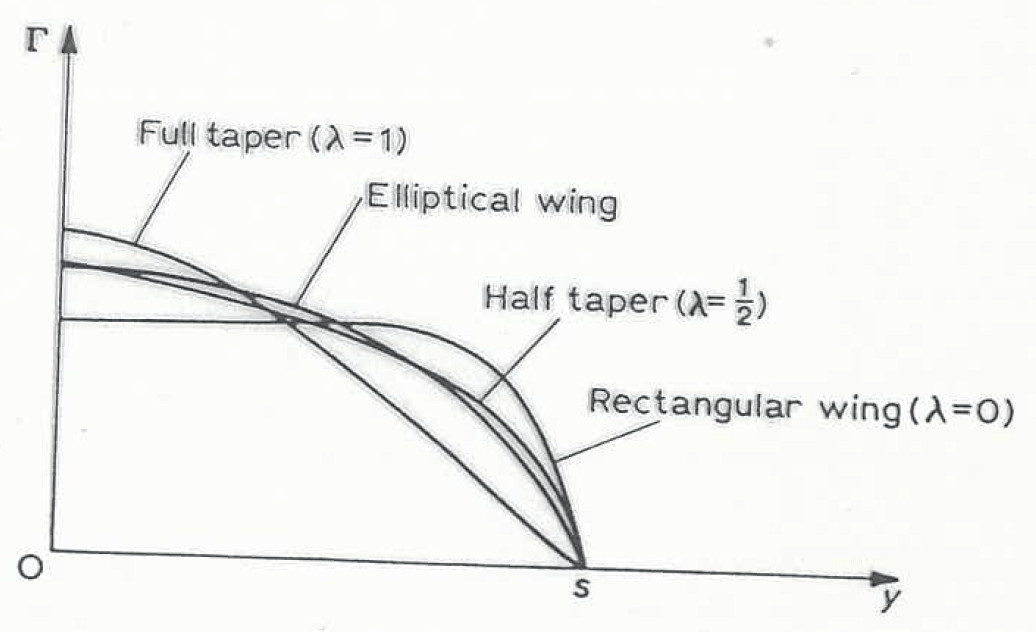
\includegraphics[scale=0.25]{ch4/23}
		\captionof{figure}{}
		\end{wrapfigure}
		a lag of $120^\circ$. The amplitude of $p(t)$ is normalised, therefore the \textbf{amplitude index} is:
		\begin{equation}
			\hat{m} = \hat{m}_a = \hat{m}_b = \hat{m}_c \qquad \mbox{linear if } \hat{m} \leq 1.
		\end{equation}
		In order to have less harmonic components, the \textbf{frequency index} must be integer, odd and multiple of 3. With such a frequency index, for each three-phase voltage the fundamental component of the output voltage is $v_{xO} = v_{xN}-V_{dc}/2$, with $x \in \{a, b, c\}$ : 
		\begin{equation}
			\hat{V}_{xO,1} = \hat{m}\frac{1}{2}V_{dc}\qquad and \qquad V_{xO,1} = \hat{m}\frac{1}{2\sqrt{2}}V_{dc}
		\end{equation}
		And the phase-to-phase voltage with a lag of $120\circ$ (e.g. $v_{ab}(t) = v_{aO}(t) - v_{bO}(t)$) :
		\begin{equation}
			\hat{U}_{1} = \hat{m}\frac{\sqrt{3}}{2}V_{dc}\qquad and \qquad U_{1} = \hat{m}\frac{\sqrt{3}}{2\sqrt{2}}V_{dc}
		\end{equation}
		In the figure, we observe unipolar phase-to-phase voltages with $m_f$ positive/negative impulsions by positive/negative alternation of the fundamental voltage. Harmonics appear near of frequencies multiples of $f_{s,p} =f_{s,T}$. There is half-wave-symmetry $\Rightarrow$ no even order harmonics. There is an additional symmetry due to the three-phase system (when $v_{ab} + v_{bc} + v_{ca} = 0$) so orders multiple of three do not appear in the phase-to-phase voltages (there are no relevant low order harmonics). 
		
	\subsection{Overmodulation and square-wave switching}
	    As in single-phase modulation, when $\hat{m}>1$ then $v_1(t)$ increases in a non-linear way. As $f_{s,T}$ is smaller there are less losses. The appearance of low order harmonics is a big disadvantage but even order harmonics and harmonics multiples of 3 remain absent from the spectre. The previous characteristic is still valid and:
		\begin{equation}
			\hat{U}_1 = \frac{4}{\pi}\frac{\sqrt{3}}{2}V_{dc}\qquad et \qquad U_1 = \frac{\sqrt{6}}{\pi}V_{dc}.
		\end{equation}
		are maximum.
		
	\subsection{Generic RLE load and phase-to-neutral voltage}
	\begin{wrapfigure}[12]{r}{5.2cm}
	\vspace{-5mm}
	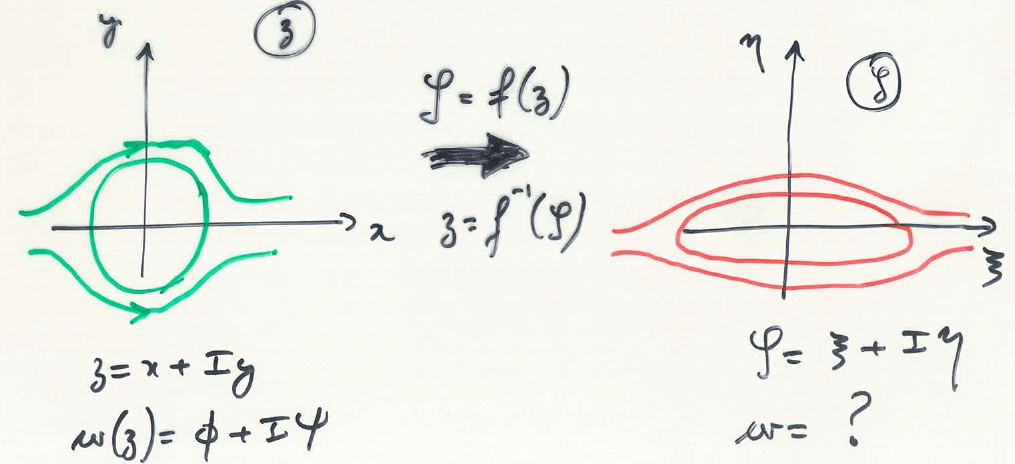
\includegraphics[scale=0.3]{ch4/28}
	\captionof{figure}{}
	\label{fig:4.22}
	\end{wrapfigure}
	If we consider a symmetric load with a star-connexion and a neuter $n$ operating according to these 3 equations :
	\begin{equation}
		v_{xn} = Ri_x + L\frac{di_x}{dt} +e_x \qquad x\in \{ a, b, c \} .
	\end{equation}			
	Depending on the application and the precision of the modelisation, the e.m.f. will be either perfectly sinusoidal or slightly distorted.  The 3 equations depend on the three-phase inverter ($V_{dc}$ + switches control).
	
	 \ \\ The addition of the 3 currents nullifies itself. If we consider that the addition of $e_x$ will also nullify (it happens often in practice), then according to the previous equations we can conclude that:
	 \begin{equation}
	 	v_{an} +v_{bn}+v_{cn} = 0
	 	\label{eq:4.38}
	 \end{equation}
	 
	 We get to the relation: 
	 \begin{equation}
	 	v_{xn} = v_{xN} - v_{nN}
	 	\label{eq:4.39}
	 \end{equation}
	 
	 \begin{wrapfigure}[12]{l}{6cm}
		\vspace{-5mm}
		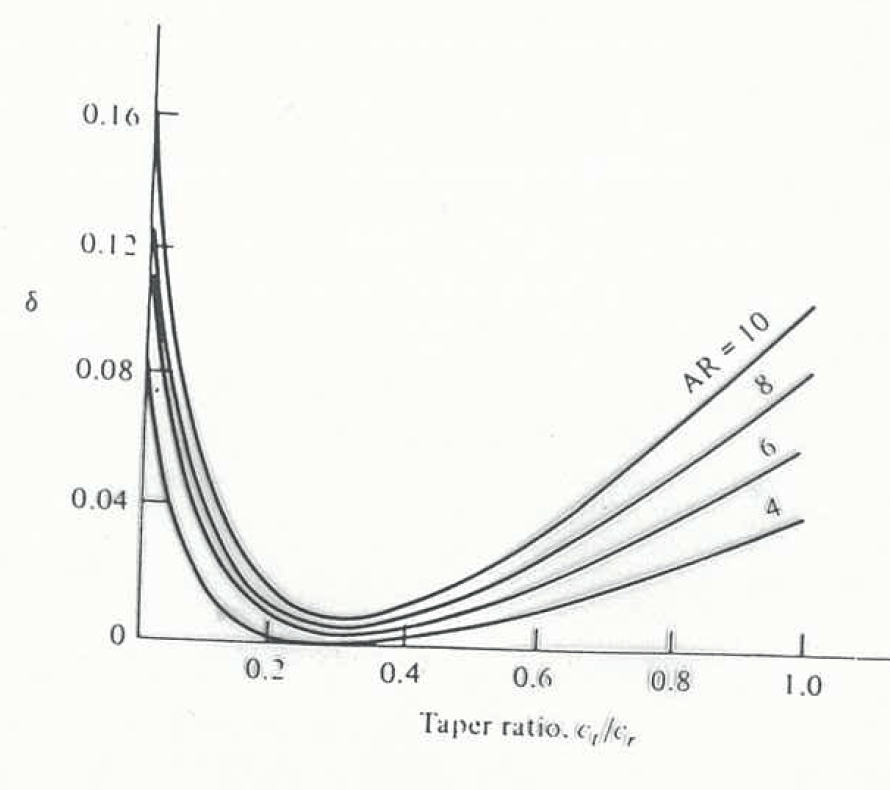
\includegraphics[scale=0.28]{ch4/24}
		\captionof{figure}{}
		\end{wrapfigure}
		where $v_{xN}$ is either 0 or $V_{dc}$, depending on the control of the leg x. This is valid if we neglect the dead time and if we suppose that semi-conductors are ideal. If we take into account the midpoint, then:
	 \begin{equation}
	 	v_{xn} = v_{xO} - v_{nO}
	\end{equation}	  
	where $v_{x0}$ is either $-V_{dc}/2$ or $+V_{dc}/2$. If we retake  \eqref{eq:4.38}, then we get:
	\begin{equation}
	\begin{aligned}
	v_{nN} &= \frac{1}{3} (v_{aN} +v_{bN}+v_{cN})\\
	v_{nO} &= \frac{1}{3} (v_{aO} +v_{bO}+v_{cO})
	\end{aligned}
	\end{equation}
	If we use \eqref{eq:4.39} we get: 
	\begin{equation}
	\begin{aligned}
	v_{an} &= \frac{1}{3} (2v_{aN} -v_{bN}-v_{cN})\\
	v_{bn} &= \frac{1}{3} (2v_{bN} -v_{aN}-v_{cN})\\
	v_{cn} &= \frac{1}{3} (2v_{cN} -v_{bN}-v_{aN})
	\end{aligned}	
	\end{equation}
	And likewise for O. All this is represented for the case of a square-wave commutation in the figure. We note that $v_x$ have discrete values $\pm \frac{1}{3}V_{dc}$ and $\pm \frac{2}{3}V_{dc}$, $v_{nN}$ takes 2 values $ \frac{1}{3}V_{dc}$ and $\frac{2}{3}V_{dc}$ and its average is $V_{dc}/2$; finally $v_{aO}=\pm \frac{1}{6}V_{dc}$ is purely an AC signal of frequency $3f$. The case of a linear PWM is in the figure under this paragraph. We can see that there are also intervals with zero voltage that will induce a lower fundamental component.
	
	\begin{center}
		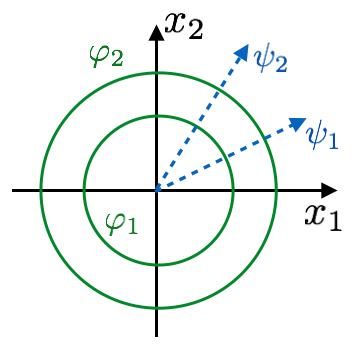
\includegraphics[scale=0.5]{ch4/25}
		\captionof{figure}{}
	\end{center}
	
	\subsection{Space vector modulation}
		\paragraph{For a given regime}\quad We introduce the space vector $\vec{v}(t)$ of the 3 phase-to-neuter voltages $v_{an}(t), v_{bn}(t)$ and $v_{cn}(t)$ as the complex number: 
		\begin{equation}
			\vec{v}(t) = \frac{2}{3} \left( v_{an}(t) + e^{j2\pi/3}v_{bn}(t)+ e^{-j2\pi/3}v_{cn}(t) \right),
		\end{equation}
	    under the hypothesis of a direct-order stead-state $a\rightarrow b \rightarrow c$. The real and imaginary parts $\alpha$ and $\beta$ are:
		\begin{equation}
			v_{\alpha}(t) = \frac{2}{3} v_{an}(t) - \frac{1}{3}(v_{bn}(t) + v_{cn}(t)) \qquad and \qquad v_{\beta}(t) = \frac{\sqrt{3}}{3}(v_{bn}(t) - v_{cn}(t)).
			\label{eq:4.44}
		\end{equation}
		The neuter n could be exchanged for any point because:
		\begin{equation}
			\vec{v}(t) = \frac{2}{3} \left( v_{am}(t) + e^{j2\pi/3}v_{bm}(t)+ e^{-j2\pi/3}v_{cm}(t) \right) + \frac{2}{3}v_{nm}(t) \underbrace{\left( 1+e^{j2\pi/3} + e^{-j2\pi/3}\right)}_{=0}. 
		\end{equation}
		We can write \eqref{eq:4.44} as function of phase-to-phase voltages if we remember that their addition nullifies itself: 
		\begin{equation}
			v_\alpha (t) = \frac{2}{3}(v_{ab}(t) - v_{ca}(t)) \qquad and \qquad v_\beta = \frac{\sqrt{3}}{3}(v_{bc}(t))= -\frac{\sqrt{3}}{3}(v_{ab}(t)-v_{v_{ca}(t)}).
		\end{equation}
		
		\paragraph{Sinusoidal regime} \quad We can prove that, for a three-phase system with three phase-to-neuter voltages of pulsation $\omega$ represented by a phasor $\underline{V}$, $\vec{v}(t) = \sqrt{2}\underline{V}e^{j\omega t}$, it can be written as follows:
		\begin{equation}
			\left\{
			\begin{aligned}
			v_{an}(t) &= \sqrt{2}V \cos (\omega t +\gamma)\\
			v_{bn}(t) &= \sqrt{2}V \cos (\omega t +\gamma - 2\pi /3)\\
			v_{cn}(t) &= \sqrt{2}V \cos (\omega t +\gamma + 2\pi /3)
			\end{aligned}
			\right.
			\qquad \Rightarrow \qquad
			\left\{ 
			\begin{aligned}
			v_\alpha (t) &= \sqrt{2}V\cos (\omega t + \gamma)\\
			v_\alpha (t) &= \sqrt{2}V\cos (\omega t + \gamma - \pi /2)
			\end{aligned}
			\right.
		\end{equation}
		
		\begin{wrapfigure}[6]{l}{4.5cm}
		\vspace{-5mm}
		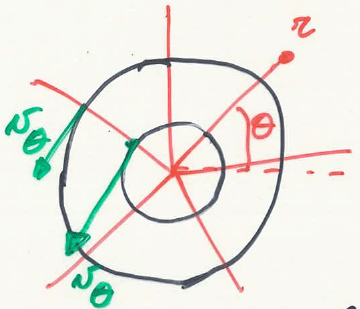
\includegraphics[scale=0.25]{ch4/26}
		\captionof{figure}{}
		\end{wrapfigure}
		$v(t)$ has a constant length $\sqrt{2}V$ that is the amplitude of the phase-to-neuter voltages and rotates at an angular velocity $\omega$. The space vector is represented in the figure, where it draws a circle of radius $\hat{V} =\sqrt{2}V$ with its center in the origin of the complex plan. \\\\\\\\
		
		\begin{wrapfigure}[6]{r}{4.5cm}
		\vspace{-5mm}
		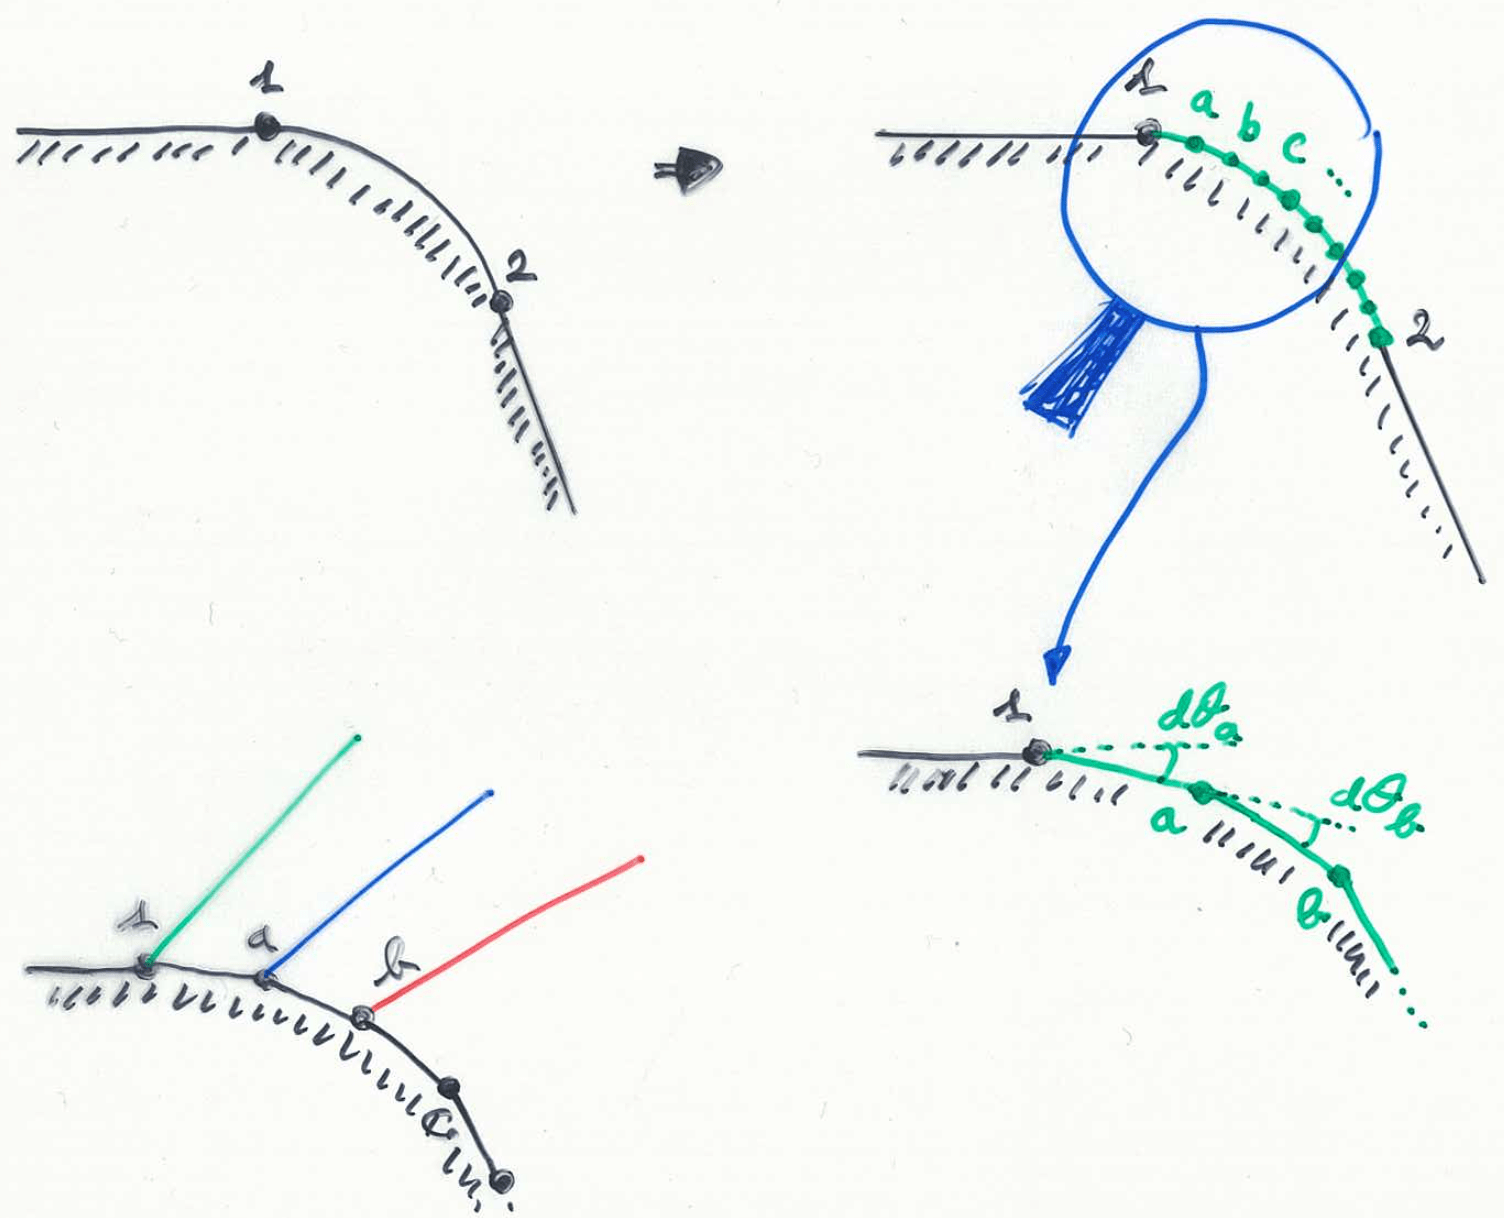
\includegraphics[scale=0.3]{ch4/27}
		\captionof{figure}{}
		\end{wrapfigure}
		\paragraph{Visualisation of the voltage space vector with an oscilloscope} \quad In practice, the auxiliary circuit in the figure facilitates the obtention of the voltages $v_\alpha$ and $v_\beta$. $m$ is therefore the midpoint of a voltage divider (e.g. resistive divider). We have: 
		\begin{equation}
			v_{am} = \frac{3}{2}v_\alpha \qquad and \qquad v_{bm} = \frac{\sqrt{3}}{2}v_\beta . 
		\end{equation}
		In the oscilloscope, if we put the output in XY format, we can get a circular locus in the particular case of a steady-state sinusoidal three-phase system.
		
		\paragraph{Three-phase inverter and voltage space vectors hexagon} \quad The three-leg voltage inverter can produce $2^3 = 8$ constant and discrete space vectors depending on the disposition of the switches: 6 nonzero space vectors(same length $60\circ$ phase shift) and 2 zero space vector. The figure to the left represents one of the combinations, the one referred to as (010). We choose for $m$ the midpoint of the DC bus. In this case the space vector is:
		\begin{equation}
			\vec{v} = \frac{2}{3} \frac{V_{dc}}{2}(-1 + 1e^{j2\pi /3}-1 e^{j2\pi /3}) = \frac{2}{3}V_{dc}e^{j2\pi /3}.
		\end{equation}
		This way we can get these 6 space vectors:
		\begin{equation}
			\vec{v}_k = \frac{2}{3}V_{dc}e^{j(k-1)\pi /3}\qquad with \qquad 1\leq k \leq 6.
		\end{equation}
		The 6 space vectors constitute the radius of an hexagon on the complex plan. Let's note that we obtain the commutation diagram of the square-wave in \autoref{fig:4.22} by going from one summit of the hexagon to another and remaining there during $T/6$. The remaining 2 are zero space vectors (they appear when both the upper and the lower switches are either closed or open). 
		\begin{center}
		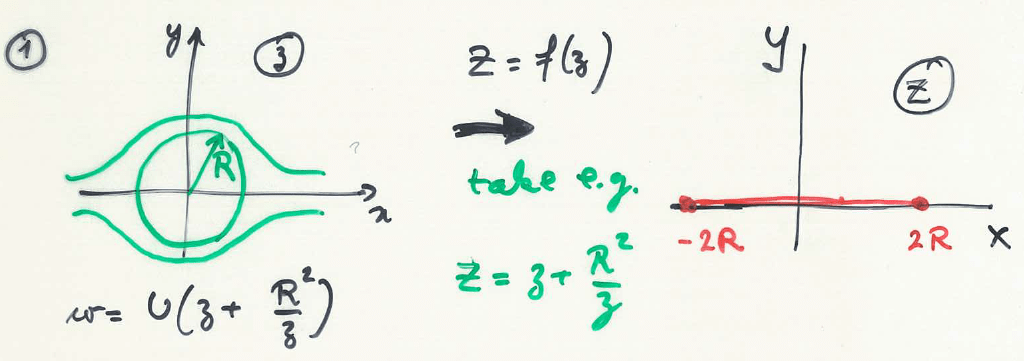
\includegraphics[scale=0.4]{ch4/29}
		\captionof{figure}{}
		\label{fig:4.27}
		\end{center}
		
		\paragraph{Space Vector Modulation} \quad (SVM) allows us to follow (in average) a space vector instruction $\vec{v}(t)$ with a given commutation period $T_s$. During each $T_s$, 4 out of 8 vectors are combined with a suitable weight in order to obtain (in average) a space vector in a certain sector $\vec{v}(t)$. For example, the vector $\vec{v}(t)$ in \autoref{fig:4.27} is obtained by combining $\vec{v}, \vec{v}_5, \vec{v}_7 = 0$ and $\vec{v}_0 = 0$: 
		\begin{equation}
			\vec{v} = \frac{T_4}{T_s}\vec{v}_4 + \frac{T_5}{T_s}\vec{v}_5 +\frac{T_7}{T_s}\vec{v}_7+ \frac{T_0}{T_s}\vec{v}_0
		\end{equation}
		with $T_4+T_5+T_7+T_0=T_s$ and $T_7=T_0$. The order in which the 4 vectors are controlled will have great influence on commutation losses.
		We can generate, in average, any space vector $\vec{v}(t)$ as long as the vector is in the hexagon. When the endpoint of the space vector $\vec{v}$ draws a circle inside the hexagon, the output voltage of the inverter doesn't have low order harmonics. The maximum rms value is obtained thanks to the radius of the circle drawn by the space vector. In fact, the radius $\hat{V}_{1,max} = V_{dc}/\sqrt{3}$. 
		
		\paragraph{Voltage range - comparison with intersective PWM} \quad We must remember that, with the intersective PWM, we avoid low order harmonics with 3 sinusoidal $m(t)$ with maximum amplitude $\hat{m}=1$, and its respective peak voltage $\hat{V}_{1,max} = V_{dc}/2$. We can get a higher value if we superpose a $3^{rd}$ order harmonic to the $m(t)$ without inducing low order harmonics on the output voltage ($\hat{V}_{1,max}=V_{dc}/\sqrt{3}$). The table hereunder comprises the different modulations.
		\begin{center}
		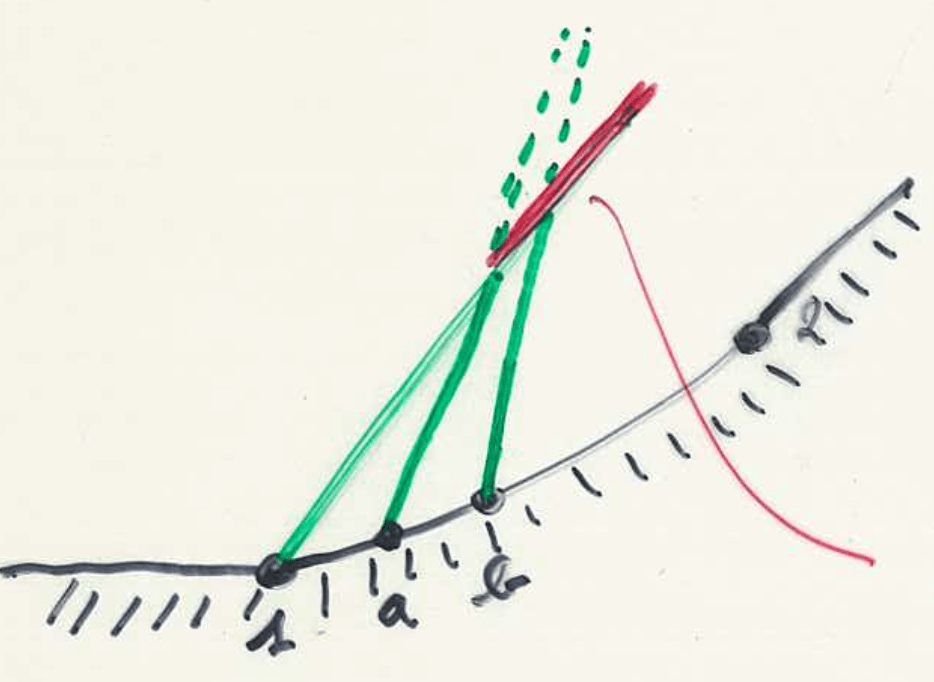
\includegraphics[scale=0.4]{ch4/30}
		\captionof{table}{}
		\end{center}
		
		Finally, we should note that the voltage capacity of the switches depends on the bus $V_{dc}$ and not on the commutation diagram. 
		
\section{Voltage control (through PWM) versus current control (through hysteresis)}
	\paragraph{Voltage converters}\quad 
	The bridges studied up to this moment can operate as inverters/rectifiers and choppers. As they are fed by a DC voltage, we can control the switches and the output voltage will be followed by the average (except commutation harmonics) as long as we don't go over the limits imposed by the DC bus and the bridge's topology. With the PWM commutation has a constant frequency. 
	
	\paragraph{Electrical drives} \quad 
	Voltage control might be useful for some electrical drives depending on the relation between voltage level, frequency in the case of AC machines and speed (at steady-state). The performance of this kind of control is poor.\\ 
	
	In order to have better performances we must control the instantaneous \textbf{electromagnetic torque} of the machine. That means controlling the currents we need to inject. By taking into account the dynamic equations of the machine we can write a current $i_{ref}$ (continuous) instruction based on the torque instruction.
	
	\paragraph{Voltage control}\quad In order to control the current, we go through either a voltage control (PWM or another, \autoref{fig:4.28}) or we act on the controllable switches of the converter depending on the difference between the desired current and the actual current (hysteresis or current control, \autoref{fig:4.29}). 
	\begin{center}
	\begin{minipage}{0.49\textwidth}
	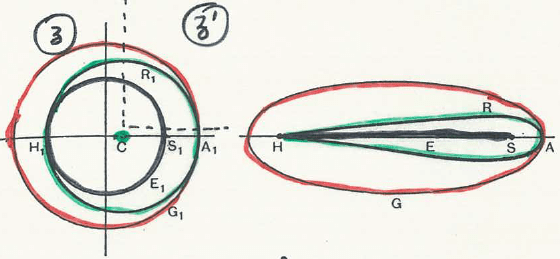
\includegraphics[scale=0.28]{ch4/31}
	\captionof{figure}{}
	\label{fig:4.28}
	\end{minipage}
	\begin{minipage}{0.49\textwidth}
	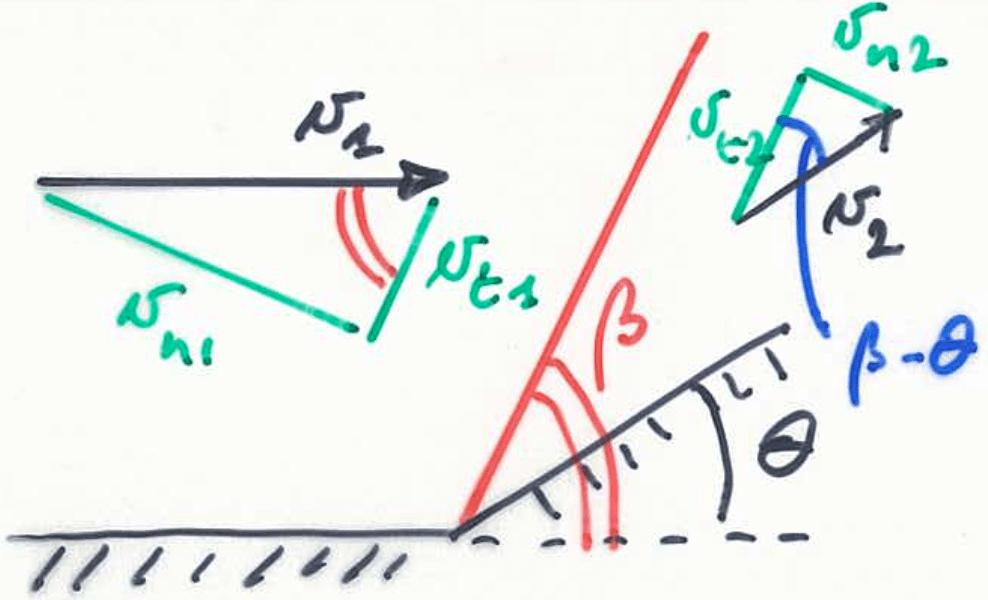
\includegraphics[scale=0.29]{ch4/32}
	\captionof{figure}{}
	\label{fig:4.29}
	\end{minipage}
	\end{center}
	
	If we do a voltage control, then the current error is translated to a voltage instruction $v_{ref}$ by means of a regulator block R set before the intersective PWM. The comparison between $p(t)$ and $m(t)$ takes place in the PWM block and the \textbf{trigger drivers} (D) control the switches.
	
	\paragraph{Current control}\quad In this case, the switches are directly controlled by the error on the current instruction. A \textbf{tolerance band} (hysteresis band) $\Delta I_{pp}$ with its center at the instruction value at that instant. If a leg furnishes a current higher than the upper limit of the tolerance band ($\Delta I_{pp}/2$ higher than the instruction), then the upper switch of the leg gets open and the lower one gets closed. When it gets lower than the lower limit of the tolerance band we open the lower switch and we close the upper one (the opposite). \\
	
	This control is quite simple but the commutation frequency is not constant because of the dependence on the parameters of our system (e.g. its inductance) and $\Delta I_{pp}$. 
	
\section{Current-source converters}
	\begin{wrapfigure}[9]{l}{6.5cm}
		\vspace{-5mm}
		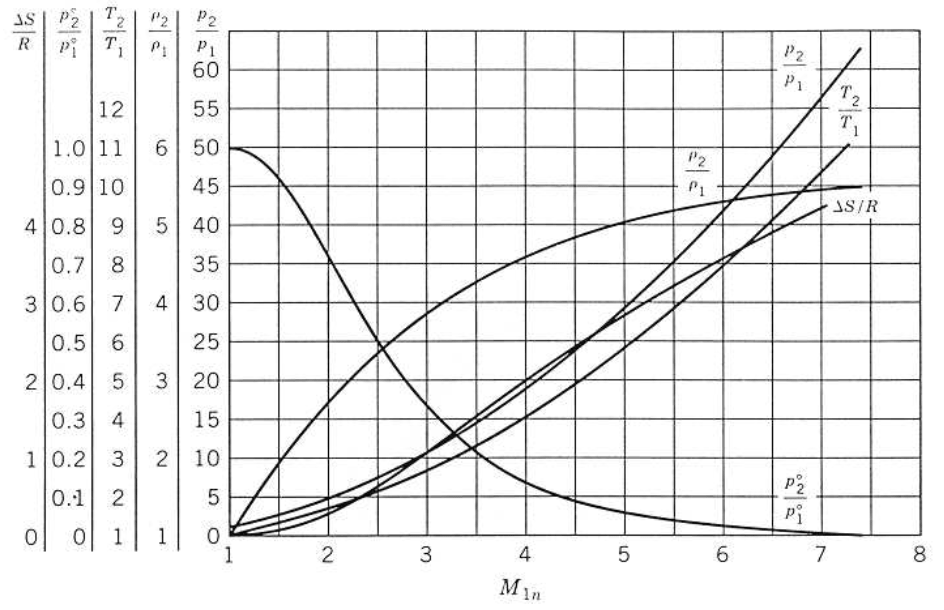
\includegraphics[scale=0.25]{ch4/33}
		\captionof{figure}{}
		\end{wrapfigure}
	We use this kind of converters for high power applications and for variable velocity control of big induction (asynchronous) or synchronous motors. An example of such a system is on the side. The DC bus comprises a big inductance L that will smooth the unidirectional current $i_{dc}(t)$. GTOs might be adequate switches for these applications because they have a large power capacity. \\
	
	The unidirectionality of the DC current $i_{dc}(t)$ allows us to do without diodes set in anti-parallel. A brief short-circuit in the leg is not a big problem anymore because the big inductance $L$ will prevent fast current variations. However, in these systems we need to avoid open circuits and the stop of the current flowing through the inductance. With a square-wave control we can employ switches with lower frequency capacities such as GTOs. \\
	
    In this system, $I_{dc}$ is fed by a thyristor rectifier. If we modify $\alpha$, we can control $V_{dc}$ and thus $I_{dc}$. If we invert $V_{dc}$ we can invert the power flux. 